\documentclass[pdftex,fontsize=12pt,a4paper,numbers=noenddot]{scrartcl}
 
% Dateiformat 
\usepackage[utf8]{inputenc}

% Sprache
\usepackage[ngerman]{babel}

% Silbentrennung
\usepackage[T1]{fontenc}  

% Serifenlose Schrift wie Arial
\usepackage[scaled]{uarial}
\renewcommand*{\familydefault}{\sfdefault}

% Zeilenabstand
\linespread{1.15}
\setlength{\parindent}{0pt} 

% Seitenränder etc
\usepackage[left=3cm,right=3cm,top=2cm,bottom=2cm,bindingoffset=0mm]{geometry}

% Bilder und Grafiken
\usepackage{graphicx}

% Kopf- und Fußzeilen
\usepackage{footmisc}
\usepackage[automark]{scrpage2} 

% Aufzählungen, Tabellen, ...
\usepackage{enumitem}
\usepackage{longtable}
\usepackage{supertabular}
\usepackage{tabularx}
\usepackage{longtable}
\usepackage{colortbl}
\usepackage{multirow}

% Nummerierung von Abbildungen
\usepackage{chngcntr}
\counterwithin{figure}{section}
\counterwithin{table}{section} 

% Schriftsatz
\usepackage{textcomp}
\usepackage{float}

%Abkürzungsverzeichnis
%Optionen:
%PrintOnlyUsed - nur genutzte Abkürzungen werden verwendet
%Withpage - im Abkürzungsverzeichnis wird die Seitenzahl eingefügt (erstes Auftreten der Abkürzung)
%\usepackage[printonlyused,withpage]{acronym}
\usepackage{acronym}

% Farben
\usepackage{xcolor}
\definecolor{blue}{RGB}{0,0,120}
\definecolor{green}{RGB}{0,153,0}
\definecolor{backcolor}{rgb}{0.9,0.9,0.9}
\definecolor{yellow}{RGB}{255,210,0}
\definecolor{gold}{RGB}{218,165,32}
\definecolor{DarkOrchid}{RGB}{92,30,123}

% Hyperlinks in der PDF
\usepackage[colorlinks, linkcolor=black]{hyperref}
\usepackage{url}

\usepackage{pdflscape}

% Einstellungen Kopf- und Fußzeile
\pagestyle{scrheadings}
\clearscrheadfoot{}
\ofoot[]{\pagemark}
\ifoot[]{TTT}
\cfoot[]{Version 0.8, \today }
\ohead[]{\headmark}
\setheadsepline[\textwidth]{1pt}

% Ebenen Nummerierungen
\setcounter{secnumdepth}{4} %Nummerierungsebenen
\setcounter{tocdepth}{4}   %Ebenen Inhaltsverzeichnis


\begin{document}

\pagenumbering{gobble} %Seiten nicht mitzählen
%TODO: Grafisch Überarbeiten
\author{Tactical Training Team}
\begin{titlepage}
	\sffamily
	\begin{tabular}{|l>{\raggedright\hspace{0pt}\arraybackslash}p{0.9\linewidth}}
		& \\
		& \Large\textbf{Tactical Training Team}\\[\baselineskip]
		& \Huge\textbf{TTT Handbuch}\\
		& \\
		& \large\today\\
		& \\
	\end{tabular}
	\pagebreak
	\begin{center}
			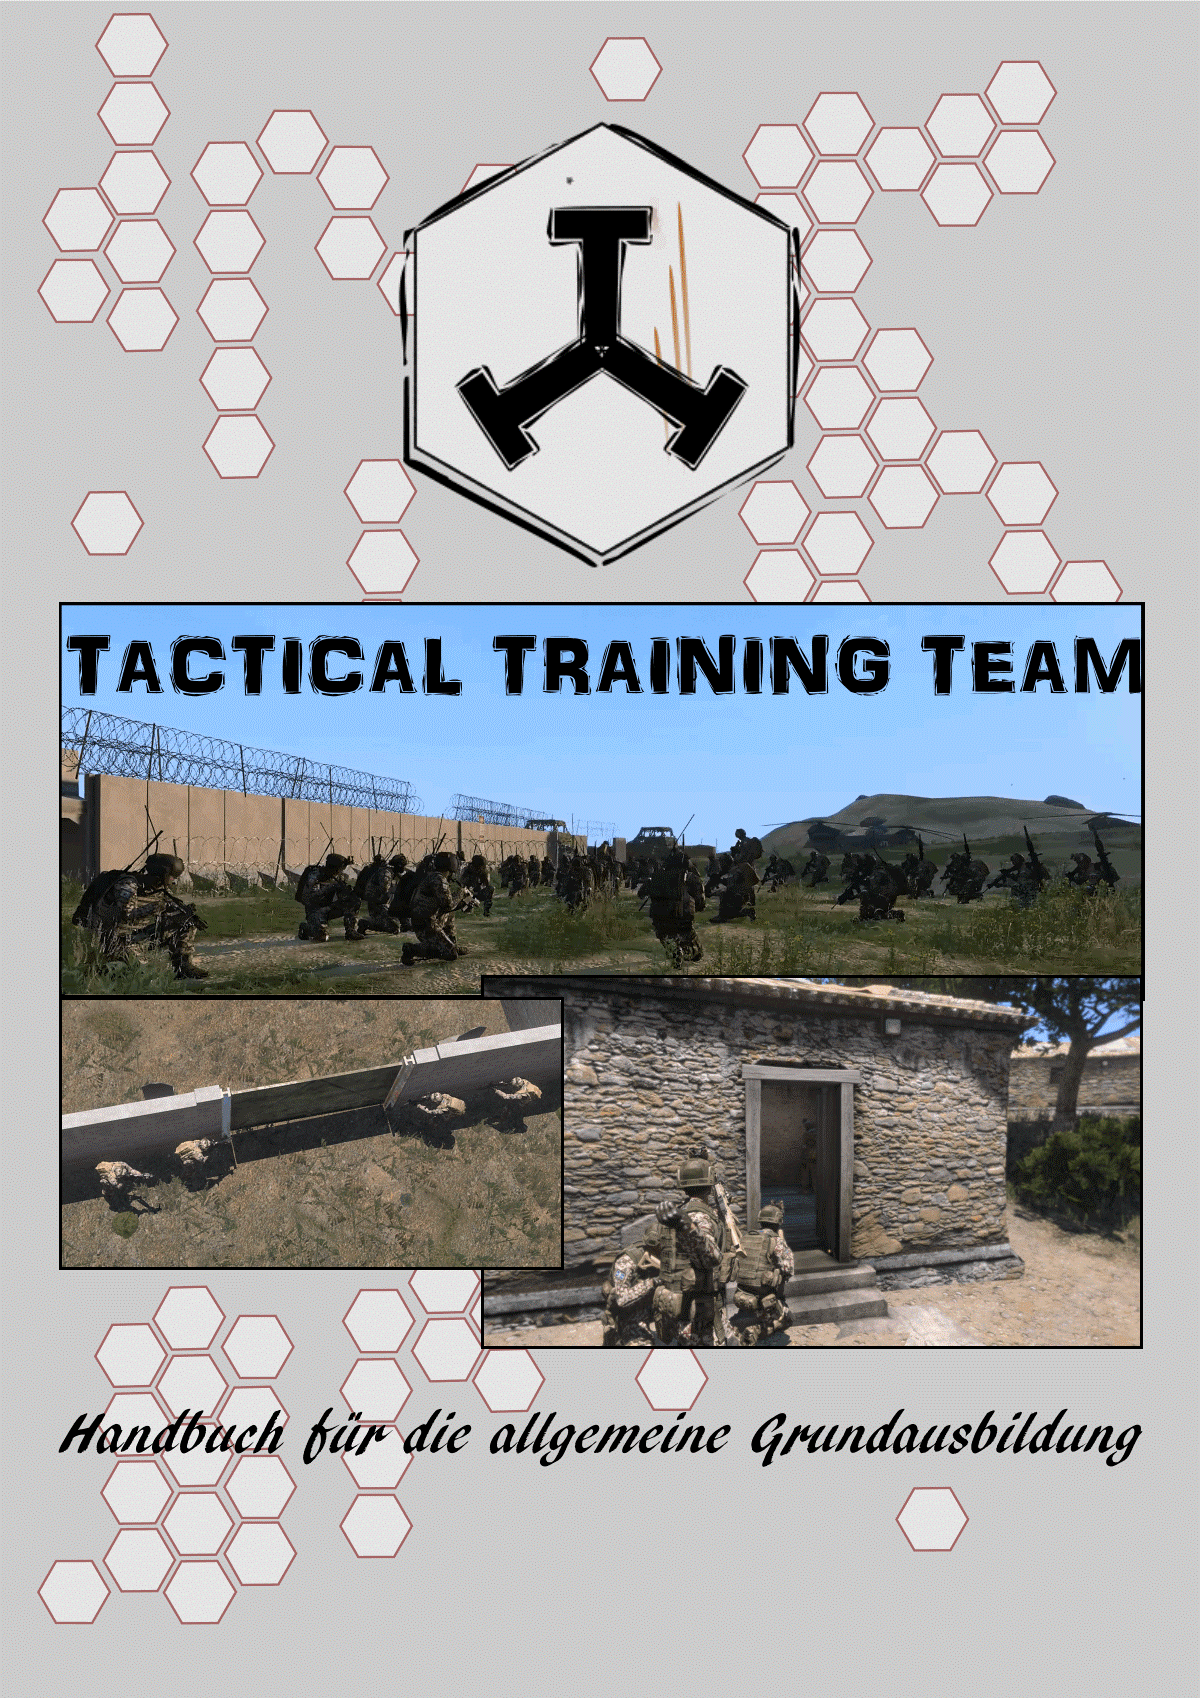
\includegraphics[width=\textwidth]{./Grafiken/Abschnitt/TTTitelbild.png}
	\end{center}
\end{titlepage}

\newpage
\pagenumbering{roman} %ab hier werden römischen Seiten als Seitenzahlen mitgezählt
\tableofcontents % Inhaltsverzeichnis

\newpage
\pagenumbering{arabic} %ab hier werden Seiten als Seitenzahlen mitgezählt
\section{Vorwort}
\subsection{Über dieses Dokument}
	Entstanden aus dem ursprünglichen, kompakten Leitfaden zur Allgemeinen Grundausbildung im \ac{TTT} soll dieses Dokument sowohl Grünschnäbeln als auch Alten Hasen zum Erlernen und Festigen aller relevanten theoretischen Grundlagen des taktischen Spiels im \ac{TTT} dienen. Es ist Leitfaden, Referenzwerk und 		Messlatte in einem Dokument vereint. Wie jedes Schriftstück zur Ausbildung sollte es \textit{aktiv} gelesen werden: der Leserin oder der Leser sollte über die vermittelten Inhalte nachdenken, sie hinterfragen, diskutieren wo nötig und gewissenhaft einprägen.\\
	Dieses Dokument lebt, es wird weiterentwickelt, überarbeitet, erweitert, gekürzt -- Anmerkungen, Vorschläge und Rückmeldungen konstruktiver Art werden nicht nur gewünscht, sondern gefordert. Ein hoher Standard im Spiel beginnt mit einem hohen Standard und Anspruch an alle Unterlagen, und jeder Spieler im \ac{TTT} ist nicht nur ständigen Verbesserung und Erweiterung seiner eigenen Fähigkeiten verpflichtet, sondern auch zur Verbesserung und Erweiterung des vermittelten Wissens. Ein aufmerksamer, geübter Schütze mag den Ausgang eines Feuerkampfs für sich entscheiden - der virtuelle Krieg wird jedoch durch Strategie, Taktik und das Wissen um das \textit{WIE} entschieden, das aus den Erfahrungen von Fehlschlägen und Triumphen herrührt. Der erste Schritt den du, lieber Leser, auf dem Weg zu einem erfolgreichen Spieler im \ac{TTT} leisten musst, ist über diese Aussage zu meditieren und sie zu verstehen.\\

\textit{Train hard, play smart!}

\newpage
\subsection{Die Grundsätze des TTT}
%TODO: Schreiben

%Truppengattungen
\section{Truppengattungen}
\subsection{Operationsleitung}
\subsection{Zugführung}

\includegraphics[width=20mm]{./Grafiken/Abschnitt/TrBraun}\quad
\includegraphics[width=20mm]{./Grafiken/Abschnitt/TrGruen}\\
Zugführung -- Trupp Grün und Trupp Braun -- befehligt Fallschirmjägertrupp Schwarz und Pioniertrupp Blau, übernimmt im Notfall medizinische Erstversorgung und koordiniert \ac{MedEvac}, \ac{CAS} und Logistik wenn benötigt. 
\subsection{Infanterie}
\subsection{Spezialkräfte}

\includegraphics[width=20mm]{./Grafiken/Abschnitt/TrGold}\\
Gold -- Fernspäher -- führt Aufklärung mit Drohnen und Scharfschützenteams und bekämpft Einzelziele mit hoher Priorität.\\\\

\includegraphics[width=20mm]{./Grafiken/Abschnitt/TrGrau}\\
Grau -- Kommando Spezialkräfte -- Spezialkräfte zur gesonderten Verwendung, welche parallel zu den regulären Kräften operieren und deren Vorgehen durch Aufklärung, Sabotage und gezielte Bekämpfung von Einzelzielen unterstützt.

\subsection{Logistik}

\includegraphics[width=20mm]{./Grafiken/Abschnitt/TrSilber}\\
Silber -- Bussard -- Stellt Fahrzeuge und Personal bereit, mit denen Transport und Logistik durchgeführt werden.
\subsection{MedEvac}

\includegraphics[width=20mm]{./Grafiken/Abschnitt/TrWeiss}\\
Weiß -- \acf{MedEvac} -- Unterstützt Operationen mit Versorgungs- und Transportkapazität für Verwundete.
\subsection{Close Air Support}
\subsection{Mechanisierte Infanterie}
\subsection{Kampfpanzer}
\subsection{Artillerie}

% Grundlagen
\section{Grundlagen}
\subsection{Formationen}
Zur Bewegung durch das Gelände verwendet man Formationen, welche der sich bewegenden Gruppe Vor- und Nachteile bieten. Sie sollten jederzeit dem Gelände sowie erwarteten oder bekannten Feindkräften angepasst werden. Die Formationen welche im TTT Verwendung finden sind der \textit{Stack}, die \textit{Kolonne} und die \textit{Schützenkette}. 

\subsubsection{Der Stack}
Der Stack ist die Sammelformation vor dem Abmarsch und als Bewegungsformation beim Einstieg in Fahrzeuge. Zudem dient er als Formation für den direkten Zugriff in Räume (siehe dazu CQB \autoref{CQB}). Grundsätzlich wird der Stack in den klassischen (engen) <<Stack>> und <<Stack weit>> unterteilt. Beim <<Stack weit>> werden die Abstände lediglich erweitert.\\
\begin{figure}[!htb]
	\centering
	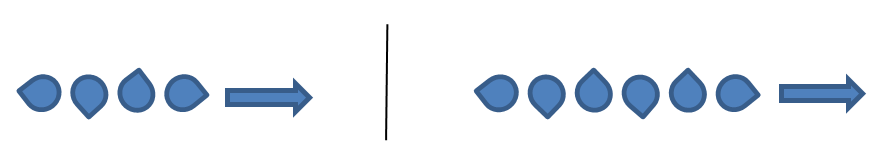
\includegraphics[width=15cm]{./Grafiken/Abschnitt/Stack.png}
	\caption{Stack 4 und 6 Mann}
\end{figure}

\subsubsection{Die Kolonne}
Die Kolonne dient als Formation im offenen Gelände und ist die Standardformation für den Marsch. Hierbei muss man zwischer einer Besonderheit im \ac{TTT} der Buddy - Kolonne und der klassischen Kolonne unterscheiden. Die Buddy - Kolonne garantiert, dass beispielsweise MG-Schütze und MG-Assistent immer zusammenbleiben, zudem verringern sie die Ausfallzahl, da sich Buddys besser gegenseitig unterstützen können. Im Gegenzug ist die klassische Kolonne weniger anfällig für Sprengsätze und Beschuss. Die Abstände zwischen den Teams sollten etwa 20 m betragen.\\
\begin{minipage}[t]{1\textwidth}
	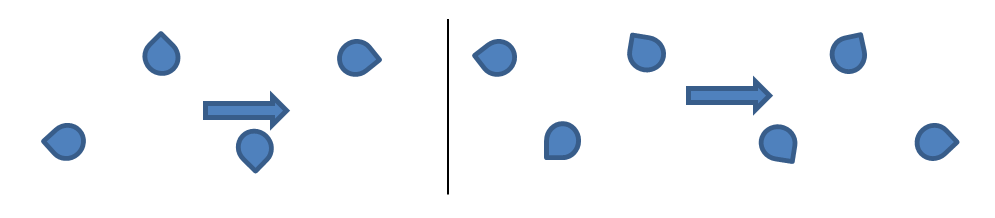
\includegraphics[width=13cm]{./Grafiken/Abschnitt/Kolonne.png}
	\label{Kolonne}
\end{minipage}
\begin{minipage}[t]{1\textwidth}
	
\includegraphics[width=13cm]{./Grafiken/Abschnitt/Buddykolonne.png}
\end{minipage}

\subsubsection{Die Schützenkette}
Die Schützenkette ist eine Formation, die zum Bezug der Stellung, in Deckung an Mauern und -- in Ausnahmefällen! -- zum Anmarsch auf einen Feind benutzen. Sie bietet maximale Feuerkraft in vermuteter Feindrichtung, lässt jedoch die Flanken und den Rückraum ungesichert. Die Schützenkette kann effizienter gestaltet werden durch entsprechende Flanken- und Rücksicherung.\\
\begin{minipage}[t]{1\textwidth}
	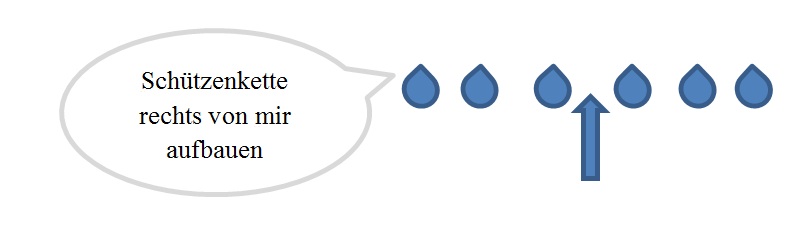
\includegraphics[width=13cm]{./Grafiken/Abschnitt/Schuetzenkette1.png}
\end{minipage}
\begin{minipage}[t]{1\textwidth}
	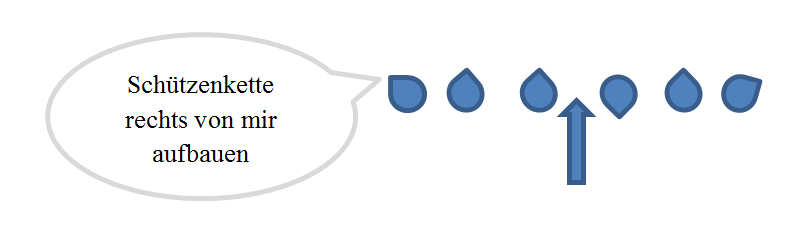
\includegraphics[width=13cm]{./Grafiken/Abschnitt/Schuetzenkette2.png}
\end{minipage}
\newpage

\subsection{Sicherungsbereiche}
	Die Sicherung wird in Bewegung immer über die Uhrzeit ausgegeben. Sowohl in Fahrzeugen als zu Fuß in Marschformationen.  Die Marschrichtung ist immer 12 Uhr. \\

\subsubsection{Rundumsicherung}
	Die Rundumsicherung bedeutet, dass 360° von dem Trupp abgesichert werden, jeder Soldat hat dazu den Auftrag, ein Viertel des \glqq Kreises\grqq abzusichern. Jeder Feind in diesem Viertel ist die Verantwortung des Soldaten. Rundumsicherung kann aus dem Marsch und in einer Stellung vollzogen werden. In Stellung geht es nicht darum, einen perfekten Kreis zu bilden – sondern sich in Deckung zu bewegen und von dort aus seinen Sektor zu sichern. Je nach Bedarf kann der Truppführer sich, um z.B. zu funken, eine 4 Mann Sicherung aufbauen lassen. \\
	Standardsicherung  – 4 Team: 
		\begin{itemize}
			\item Nr.1 sichert auf 12 Uhr 
			\item Nr.2 sichert auf 9 Uhr 
			\item Nr.3 sichert auf 3 Uhr 
			\item Nr.4 sichert auf 6 Uhr 
		\end{itemize}

		\begin{figure}[htbp]
			\centering
			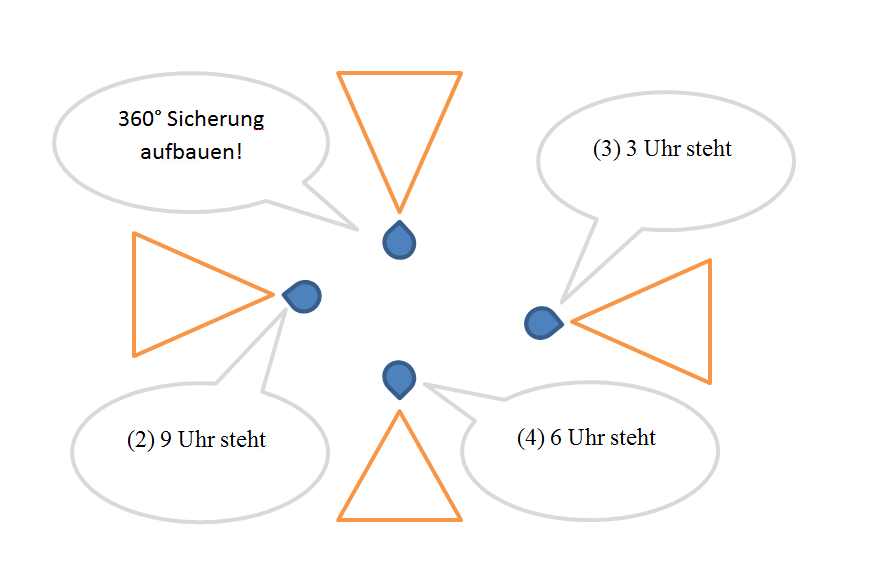
\includegraphics[width=15cm]{./Grafiken/Abschnitt/360er.png}
			\caption{4 Mann 360er}
		\end{figure}

	Standardsicherung – 6 Team: 
		\begin{itemize}
			\item Nr.1 sichert auf 12 Uhr 
			\item Nr.2 sichert auf 9 Uhr 
			\item Nr.3 sichert auf 3 Uhr 
			\item Nr.6 sichert auf 6 Uhr
			\item Nr.4 und Nr.5 springen ein bzw. unterstützen Schwerpunkte. Nr.1 kann die Verantwortung für die 12 Uhr beispielsweise an die Nr.2 abgeben – in der Stellung kann das MG auf einen Schwerpunkt verlegt werden (aus der ein Feind erwartet wird). 
		\end{itemize}

		\begin{figure}[htbp]
			\centering
			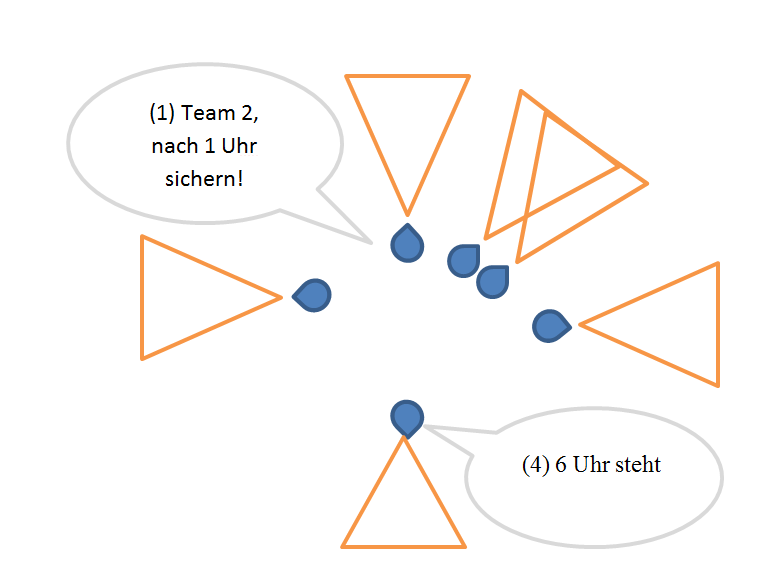
\includegraphics[width=15cm]{./Grafiken/Abschnitt/360erFS.png}	
			\caption{6 Mann 360er mit Feuerschwerpunkt}
		\end{figure}

		\begin{figure}[htbp]
			\centering
			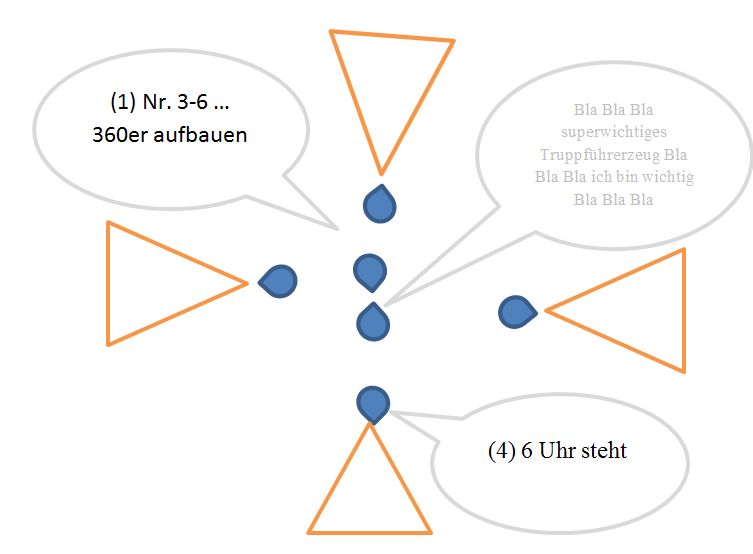
\includegraphics[width=15cm]{./Grafiken/Abschnitt/360erOTF.png}
			\caption{6 Mann 360er entlastetes Führungsteam}
		\end{figure}

\subsubsection{180°-Sicherung}
	Die 180-Grad-Sicherung ist eine Halbkreis-Sicherung. Wird in der Regel an Mauern angewandt – oder in einer Stellung, um ein zu beobachtendes Gelände abzusichern, wenn der Rückraum als absolut sicher gilt. Zu beachten ist, dass die 180° Sicherung nicht unmittelbar an der Mauer sondern etwa 1m entfernt aufgebaut wird. So können einzelne Soldaten oder Trupps hinter der Sicherung kreuzen, ohne in den eigenen Feuerbereich treten zu müssen. \\
	\begin{figure}[htbp]
		\centering
		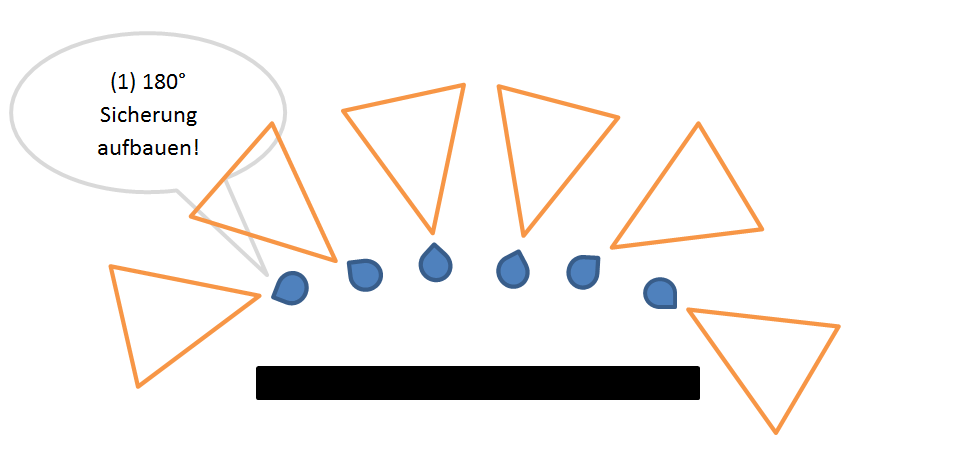
\includegraphics[width=15cm]{./Grafiken/Abschnitt/180er.png}
		\caption{180° Sicherung an Mauer}
		\end{figure}
\newpage
\newpage
\subsection{Von der Bewegung}
%TODO: Skylining, Karte lesen, ...
	\begin{center}
		\textit{Maneuvering with an army is advantageous;\\ with an undisciplined multitude, most dangerous.}
	\end{center}
	\vspace{12pt}

	Die Schlagkraft einer Truppe wird durch ihre Feuerkraft und ihre Mobilität bestimmt. Das Gelände zu kennen, es lesen zu können und sich korrekt sowohl alleine als auch im Trupp zu bewegen erfordert Kenntnis, Erfahrung und Übung. In diesem Abschnitt soll daher auf die Bewegung eingegangen werden.\\ 

	Grundsätzlich gilt, dass eine Bewegung von folgenden Faktoren bestimmt wird:
	\begin{itemize}
		\item Gelände -- Einen Bergkamm zu erreichen kann langwierig sein, und weitläufige freie Flächen sind zu meiden: eine Bewegung setzt eine 	entsprechende Vorkenntnis von Gelände und Erfahrung im Umgang mit der Karte voraus (siehe entsprechendes Kapitel).
		\item Trupp -- Je nach dem, welche Truppgröße und -zusammensetzung vorhanden ist, sind unterschiedliche Faktoren entscheidend: Tragen die Soldaten schwere oder leichte Lasten? Ist man zu viert oder sind es zwei Trupps die sich bewegen? Muss man Verwundete verlegen? 
		\item Verbündete Kräfte -- Befinden sich verbündete Truppen oder Fahrzeuge in der Nähe, welche Platz zum Manövieren benötigen? Zu dicht gedrängte Formationen laden zu Beschuss durch Artillerie ein -- stehe ich zu dicht an meinen Kameraden? Sichere ich in die richtige Richtung? Sichern wir in alle Richtungen?
		\item Feindliche Kräfte -- Welche feindlichen Kräfte sind wo zu erwarten? Wurden sie aufgeklärt, oder ist man sich unsicher wer das Territorium hält?
		\item Ziel der Bewegung -- Keine Bewegung ohne Ziel! Wo soll es hingehen? Was ist der Auftrag dort? Welcher Zeitrahmen steht zur Verfügung?
	\end{itemize}
	Egal ob man nun über ein Stoppelfeld zur nächsten Deckung hetzt, sich langsam durch eine Siedlung arbeitet oder in eine Stellung am Waldrand gleitet: es gibt Grundregel und Dinge, die jeder Soldat wissen sollte. Dazu gehören Bewegungsarten, Formationen und grundsätzliches zum Umgang mit der Waffe während der Bewegung.

\subsubsection{Bewegungsarten}
	Man unterscheidet zwischen folgenden Bewegungsarten:
	\begin{itemize}
		\item Gleiten -- Tiefste Forstbewegungsart, das Kriechen. Geschieht meist langsam um sich anzuschleichen oder eine extrem flache Silhouette zu bieten.
		\item Geduckt -- Schneller als das Gleiten, ermüdet den Soldaten rasch und passiert meist intuitiv während Bewegung hinter Deckung.
		\item Gehen -- Aufrechtes Gehen, typische Bewegungsart wenn längere Strecken überbrückt werden müssen
		\item Sprung -- Schnelles Rennen, meist zur nächsten Deckung oder um eine Distanz schnell zu überbrücken
	\end{itemize}

\subsubsection{Sicherungsbereiche}
	Während der Bewegung hat jedes Mitglied eines Trupps in eine bestimmte Richtung zu sichern. Dabei gelten für den 4-Mann-Trupp folgende Sicherungsbereiche:
	\begin{itemize}
		\item Nr.1 sichert auf 12 Uhr 
		\item Nr.2 sichert auf 9 Uhr 
		\item Nr.3 sichert auf 3 Uhr 
		\item Nr.4 sichert auf 6 Uhr 
	\end{itemize}
	Und für den 6-Mann-Trupp:
	\begin{itemize}
		\item Nr.1 sichert auf 12 Uhr 
		\item Nr.2 sichert auf 10 Uhr 
		\item Nr.3 sichert auf 2 Uhr 
		\item Nr.4 sichert auf 4 Uhr 
		\item Nr.5 sichert auf 8 Uhr
		\item Nr.6 sichert auf 6 Uhr 
	\end{itemize}

\subsubsection{Umgang mit der Waffe}
	Ständig bereit zu sein, ein Feuergefecht aufzunehmen kann aus mehreren Gründen unpraktisch oder sogar gefährlich sein. Daher gilt grundsätzlich die Waffe während des Marsches herunterzunehmen und erst in den Anschlag zu nehmen, wenn eine von folgenden Bedingungen zutrifft:
	\begin{itemize}
		\item Es muss ein erkannter Feind bekämpft werden.
		\item Die Waffe muss eingewiesen werden oder die Optik soll zur Aufklärung genutzt werden.
		\item Feindliche Kräfte auf Tuchfühlung (im Umkreis von 10m)
		\item Es wurde liegend oder stehend eine Stellung bezogen oder Sicherungsbereiche benannt.
	\end{itemize}

	In allen anderen Fällen ist die Waffe unten zu halten. In einer Basis ist sie zudem zu \textit{sichern}! \\

	Die Waffe gesenkt zu haben hat zahlreiche Vorteile:
	\begin{itemize}
		\item Das Sichtfeld ist deutlich größer.
		\item Die Wahrscheinlichkeit von Beschuss eigener Kräfte und dem Verraten der Position durch versehentliches Abfeuern der Waffe ist geringer.
		\item Die Ausdauer leidet weniger und man bewegt sich schneller.
	\end{itemize}
	Die Waffe erhoben zu haben hat einige Nachteile:
	\begin{itemize}
		\item Entwicklung eines Tunnelblicks: Der Träger blickt nur noch in eine Richtung (meist vorn und eventuell sogar noch durch die Optik)
		\item Der Soldat bewegt sich langsamer und ermüdet schneller
		\item Der Soldat gefährdet eigene Kameraden!
	\end{itemize}
	Es gilt zudem, das \textit{unter keinen Umständen} die Waffe auf eigene Kräfte gerichtet werden!

	\paragraph{Kreuzen}
		Unter \textit{Kreuzen} versteht man das Queren oder Kreuzen einer Feuerlinie eines Kameraden. Wo immer möglich ist dies zu vermeiden. Das gilt ganz besonders für Fahrzeuge, dort ist auch eine mögliche Bewegungsrichtung (nach vorn / nach hinten) jederzeit frei zu halten. Es hilft ungemein, bereits sofort nach dem Beziehen einer Stellung zu überprüfen, ob die Kameraden immer noch entsprechend manövrieren können. Wann immer man doch Kreuzen muss, ist dies verbal und früh genug anzukündigen: \textbf{\glqq Achtung, ich kreuze!\grqq}

	\paragraph{Annäherung an eigene oder verbündete Kräfte}
		Um sich an befreundete Truppen anzunähern, sollten diese möglichst durch Funk und durch persönliche Ansprache (ähnlich dem Kreuzen) gewarnt werden. Idealerweise gibt man die Annäherungsrichtung mit dazu an.\\

%TODO Tabelle optimieren (Multirow)
\subsubsection{Vokabular der Bewegung}
	\begin{longtable}{|p{0.4\linewidth} | p{0.6\linewidth} |}
		\caption[Vokabular Bewegung]{Begriffe der Bewegung} \\
		\hline
		\textbf{Begriff} & \textbf{Bedeutung} \\
		\hline
		Bereitmachen zum Sprung / Bereit zum Sprung & \\
		\hline
		Sprung auf, Marsch Marsch! & \\
		\hline
		Verschieben & \\
		\hline
		Verlegen & Bewegen über eine lange Strecke \\
		\hline
		Ausweichen & Lösen von feindlichen Kräften, meist Rückzug zu besser zu verteidigenden Position, oft mit Ablenkungen oder Deckungsfeuer kombiniert.\\
		\hline
	\end{longtable}
\newpage
\subsection{Richtig Funken und Kommunizieren im Trupp}

	Zum generellen Gebrauch des Funkgeräts sei auf den TFAR-Mod \autoref{TFAR} verwiesen. Weiterhin sollte man die eigene Stimmlautstärke nicht unbedingt auf \glqq Laut\grqq\, (\glqq yelling\grqq) stellen. Das dient dazu bei mehreren eng geführten Trupps nicht bis zum anderen Trupp rüber zu schreien.\\
	Grundsätzlich sollten alle wichtigen Meldungen dem Truppführer über die Trupp interne Funkfrequenz mitgeteilt werden.\\

\subsubsection{Kontakmeldungen}
	Kontaktmeldungen  sollten möglichst nach einem bestimmten Schema ablaufen.  Auch hier gilt im Gefecht wird nicht jede Kontaktmeldung perfekt sein. Dennoch sollte man sich an dieser Meldeform möglichst nah orientieren.
		\begin{itemize}
		\item <<Kontakt>> oder <<Freunde>>
		\item Anzahl 
		\item Was
		\item Wo (grobe Richtung, Landmarke, Landmarken ggf. verfeinern, genaue Grad zahl) 
		\item Entfernung
		\item  weitere Verfeinerung wie zum Beispiel Bewaffnung, Alarmzustand (heiß oder kalt)
	\end{itemize}

	Beispiele:\\
	<<Kontakt \dots 1 feindlicher \acs{SPZ} \dots auf 4 Uhr \dots Rechts über der Hütte \dots auf 95° \dots ca. 500m>> \\
	<<Kontakt \dots 3 Infanteristen \dots auf 1 Uhr \dots Kommen über den Hügel \dots bei 25° \dots ein \acs{MG} \dots ca. 300m \dots kalt>> \\

\subsubsection{Funkgespräch unterbrechen}
	Um eine aktuell durchgeführte Funkmeldung oder Gespräch zu unterbrechen, um eine Meldung abzusetzen von höherer Priorität, oftmals Feindkontakt, hat sich ein kurzes <<Break, Break>> oder <<Check, Check>> als sinnvoll heraus gestellt. \\
	Beispiel: \\
	TF: <<Wir gehen folgendermaßen vor Bud…>>  \\
	TM: <<Break, Break>> \dots <<Kontakt feindlicher Trupp auf 2 Uhr  100m nähert sich>> \dots  \\
	TF: <<Verstanden, Feuer frei>> \\

\subsubsection{sonstige Meldungen}
	Bei betreten oder verlassen von Fahrzeugen wird sich kurz und prägnant gemeldet das man dieses entsprechend betreten oder verlassen hat, damit erhält der TF die Information wo sein Trupp sich befindet und die Truppmitglieder wissen wie sie sich zu verhalten haben. (Erst wenn 3 meldet das er sitzt kann 2 aufsitzen) \\
	Beispiel:  <<3, Sitzt>> \\

	Meldungen über aufgebaute Sicherung können sehr nützlich sein um dem TF über den Status der Sicherung zu empfehlen. \\
	Beispiel: << Hier 6, Sicherung nach 6 Uhr steht>> \\

	Das letzte Trupp Mitglied (üblw. die Nr.6) meldet den Status der Bewegung. \\
	Beispiel: \\
	TF: <<Im Stack Marsch>> \\
	6: <<Trupp in Bewegung>>  \\
	Statusmeldung und durchzählen. \\
	Nach heftigen, ggf. unübersichtlichen Feindbeschuss ist es sinnvoll den Status des Trupps abzufragen. Sollte der Truppführer nicht erreichbar sein kann auch ein Trupp Mitglied die Statusabfrage anordnen. \\
	Es wird generell von 1 an heruntergezählt. (Wenn 1 die Statusmeldung  anordnet entfällt die Meldung der 1 i.d.R.)  \\
	Aufbau der Meldung: \\
	<<Nummer, Gesundheitsstatus, ggf. Besonderheiten>>  \\
	Beispiel:\\
	 <<1 hier 5, Kommen>> \dots (keine Reaktion)\\  
	 <<Hier 5, Trupp Status durchgeben>> \dots (kurz warten 1 und 2 melden sich nicht)\\ <<Hier 3, Status Rot>> \dots\\ 
	 <<Hier 4, Status Grün, zwei Verletzte auf dem Hügel>> \dots usw. \\

\subsubsection{Wichtigste Funkabkürzungen und Begriffe}
	\begin{tabular}{|p{2cm}|p{4cm}||p{3cm}|p{4cm}|} \hline
		\acs{SPZ}	& \acl{SPZ}	& Standby	& Bitte warten \\ \hline 
		\acs{KPZ}	& \acl{KPZ}	& Kalt		& keine Gegner, Gegner haben uns nicht erkannt \\ \hline
		\acs{AA}	& \acl{AA}	& Heiß 		& Gegner eröffnen Feuer, haben uns entdeckt \\ \hline
		\acs{AT}	& \acl{AT}	& \acs{OPL}	& \acl{OPL} \\ \hline
		\acs{MG}	& \acl{MG}	& \acs{CAS}	& \acl{CAS} \\ \hline
	\end{tabular}



\subsection{Fahrzeuge}
\subsubsection{Auf- und Ab sitzen}
	Fahrzeuge werden in umgekehrte Trupp Reihenfolge betreten. (Siehe auch \glqq Richtig Funken und Kommunizieren im Trupp\grqq)
	
\subsubsection{Sicherungsbereich}
	Der Sicherungsbereich nach Verlassen des Fahrzeuges entspricht den Standsicherungsbereichen für  Trupps (siehe Kolonne \autoref{Kolonne}, Standartsicherung 360°). Mehrere Trupps können sich z.B. 180° Sicherungsbereiche abstimmen. \\
	Kommando Verlassen:  Alle Truppteile verlassen das Fahrzeug \\
	Kommando Absitzen: Schütze bleibt, Fahrer bleibt in Nähe am Fahrzeug, Rest baut Sicherung auf.\\
	
	Wichtig:
	\begin{itemize}
		\item Bewegungskorridor vor und hinter dem Fahrzeug immer frei lassen\\ 12 Uhr ist immer die Fahrzeugfront
		\item Ein Fahrzeug in ARMA ist keine Deckung, wenn der Gegner AT-Waffen besitzt
		\item Abstand halten:\\ Wenn nicht anders befohlen, 20 Meter Abstand vom Fahrzeug\\ Fahrzeuge tendieren zum Explodieren, bieten schlechte Deckung und brauchen zudem jederzeit Platz für Manöver
	\end{itemize}
	\begin{figure}[htbp]
		\centering
		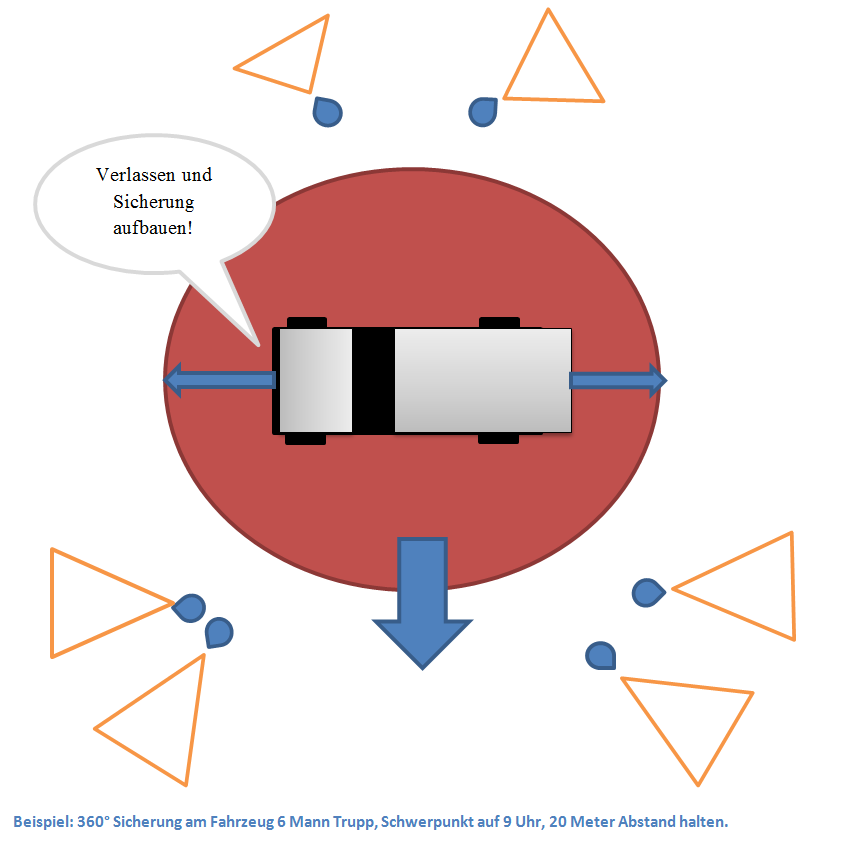
\includegraphics[width=15cm]{./Grafiken/Abschnitt/Fahrzeug_verlassen.png}
		\caption{Absitzen und Sicherung beim Fahrzeug}
	\end{figure}

\subsection{Erste Hilfe}
\subsection{Verhalten bei Feindkontakt}

%Fortgeschrittenes
\section{Fortgeschrittenes}
\subsection{Führen}
\subsubsection{Führen als Operationsleitung}
\subsubsection{Führen als Zugführer}
\subsubsection{Führen als Truppführer}
\subsection{Logistik / MedEvac anfordern (5-Liner)}

\subsection{Close Air Support anfordern}
\subsubsection{5-Liner}
\subsubsection{9-Liner}

\subsection{Artillerie anfordern (5-Liner)}
\newpage
\subsection{CQB}
\label{CQB}
\newpage

\section{Hubschrauber für Infanteristen}
\label{HuFIn}

\subsection{Hubschrauber im Einsatz}
	Pro: 
		\begin{itemize}
			\item Observation im Bereich
			\item Aufnehmen und Absetzen von Trupps
			\item Tarnung
			\item Rapid Reaction
			\item \ac{CAS}
		\end{itemize}

	Contra: 
		\begin{itemize} 
			\item Größere Verwundbarkeit (größeres Waffenkontingent)
			\item Laut
		\end{itemize}

\subsection{Aufgaben der Infanterie im Hubschrauber}
	Aufgabe der Infanterie im Flug ist es nach allen Bedrohungen Ausschau zu halten. Sei es Gewehrfeuer, Raketen, Positionen feindl. Kräfte, Hindernissen oder jeglicher anderer Gefahr für das Fahrzeug. Der Pilot ist immer zu informieren und auf dem Laufenden zu halten! Überflüssige Gespräche sollten vermieden werden.

\subsection{Koordination}
	Bevor es in den Einsatz geht sind Vorkehrungen zu treffen. 
		\begin{itemize} 
			\item Welcher Trupp kommt in welchen Hubschrauber? 
			\item Welcher Hubschrauber geht zu welcher \ac{LZ}? 	
			\item Die Kräfte sind möglichst gleich und redundant zu verteilen wenn möglich.
		\end{itemize}

	Bei Abholung bestimmt der Truppführer, wenn benötigt bzw. möglich, einen Einweiser und das letzte Sicherungsglied.

\subsection{Bereitstellen einer \acf{LZ}}
	Eine ideale \ac{LZ} bietet genug Deckung, sowohl für den Trupp als auch für den Hubschrauber. Ein minimale Landefläche beträgt $25m * 25m$ (ohne viele Hindernisse) und in dieser eine absolut freie Fläche von minimal $5 * 5$ Meter. Dies kann je nach Hubschrauber variieren. Je flacher das Gelände ist, desto weiter muss der Hubschrauber von feindlichen Kräften entfernt landen um die Sicherheit zu garantieren. Ein hügeliges Gelände erlaubt nähere Landemanöver, wenn das Terrain eine Deckung des Hubschraubers erlaubt. \\
	\begin{minipage}[t]{1\textwidth}
		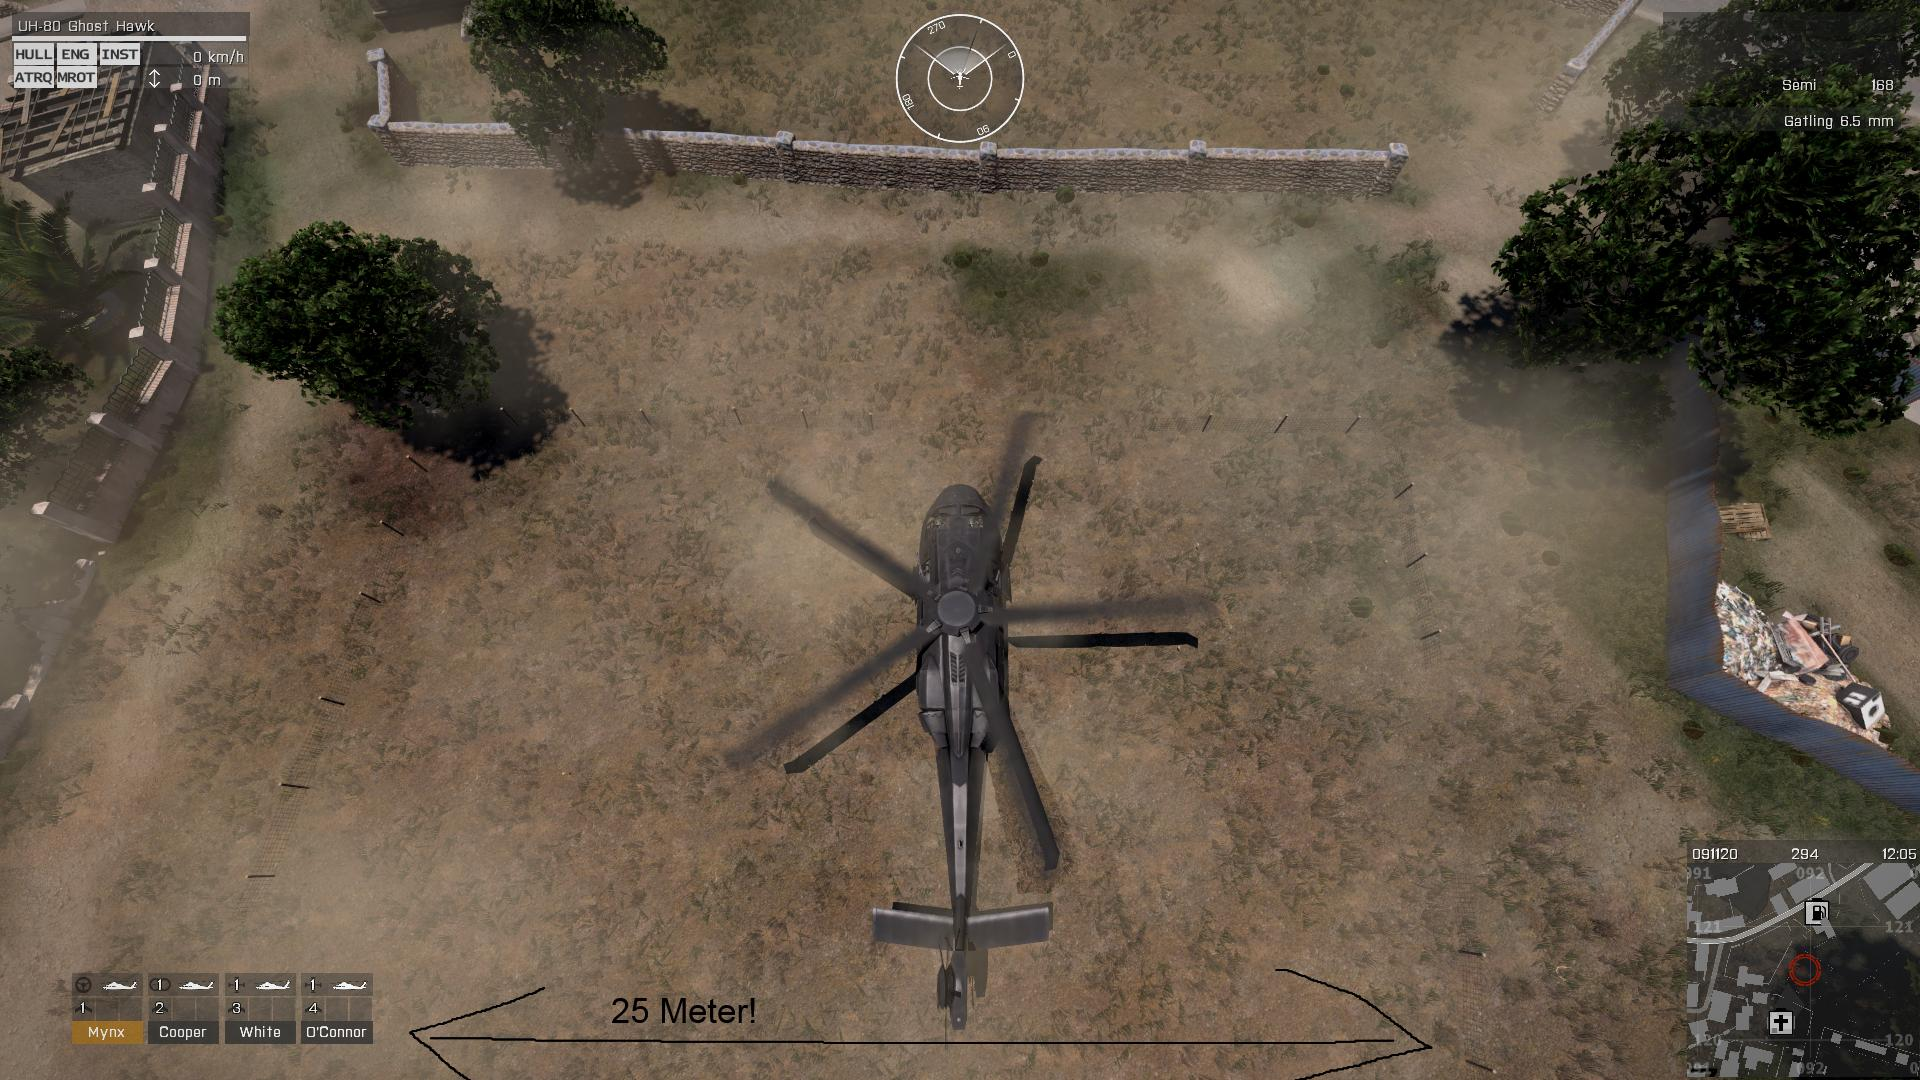
\includegraphics[width=\textwidth]{./Grafiken/Hubschrauber/Landezone.jpg}
	\end{minipage}

	Für den Anflugbereich wird angestrebt, einen möglichst sicheren (am besten Unsichtbaren) Anflugbereich zu ermöglichen. Trupps werden wenn möglich >>direkt in der Deckung<< abgeladen oder aufgenommen. Es ist erstrebenswert das der Hubschrauber während des Landemanövers über möglichst viel Deckung verfügt. Je näher am Gegner gelandet werden muss, desto größer ist die Gefahr. \\
	\begin{minipage}[t]{1\textwidth}
		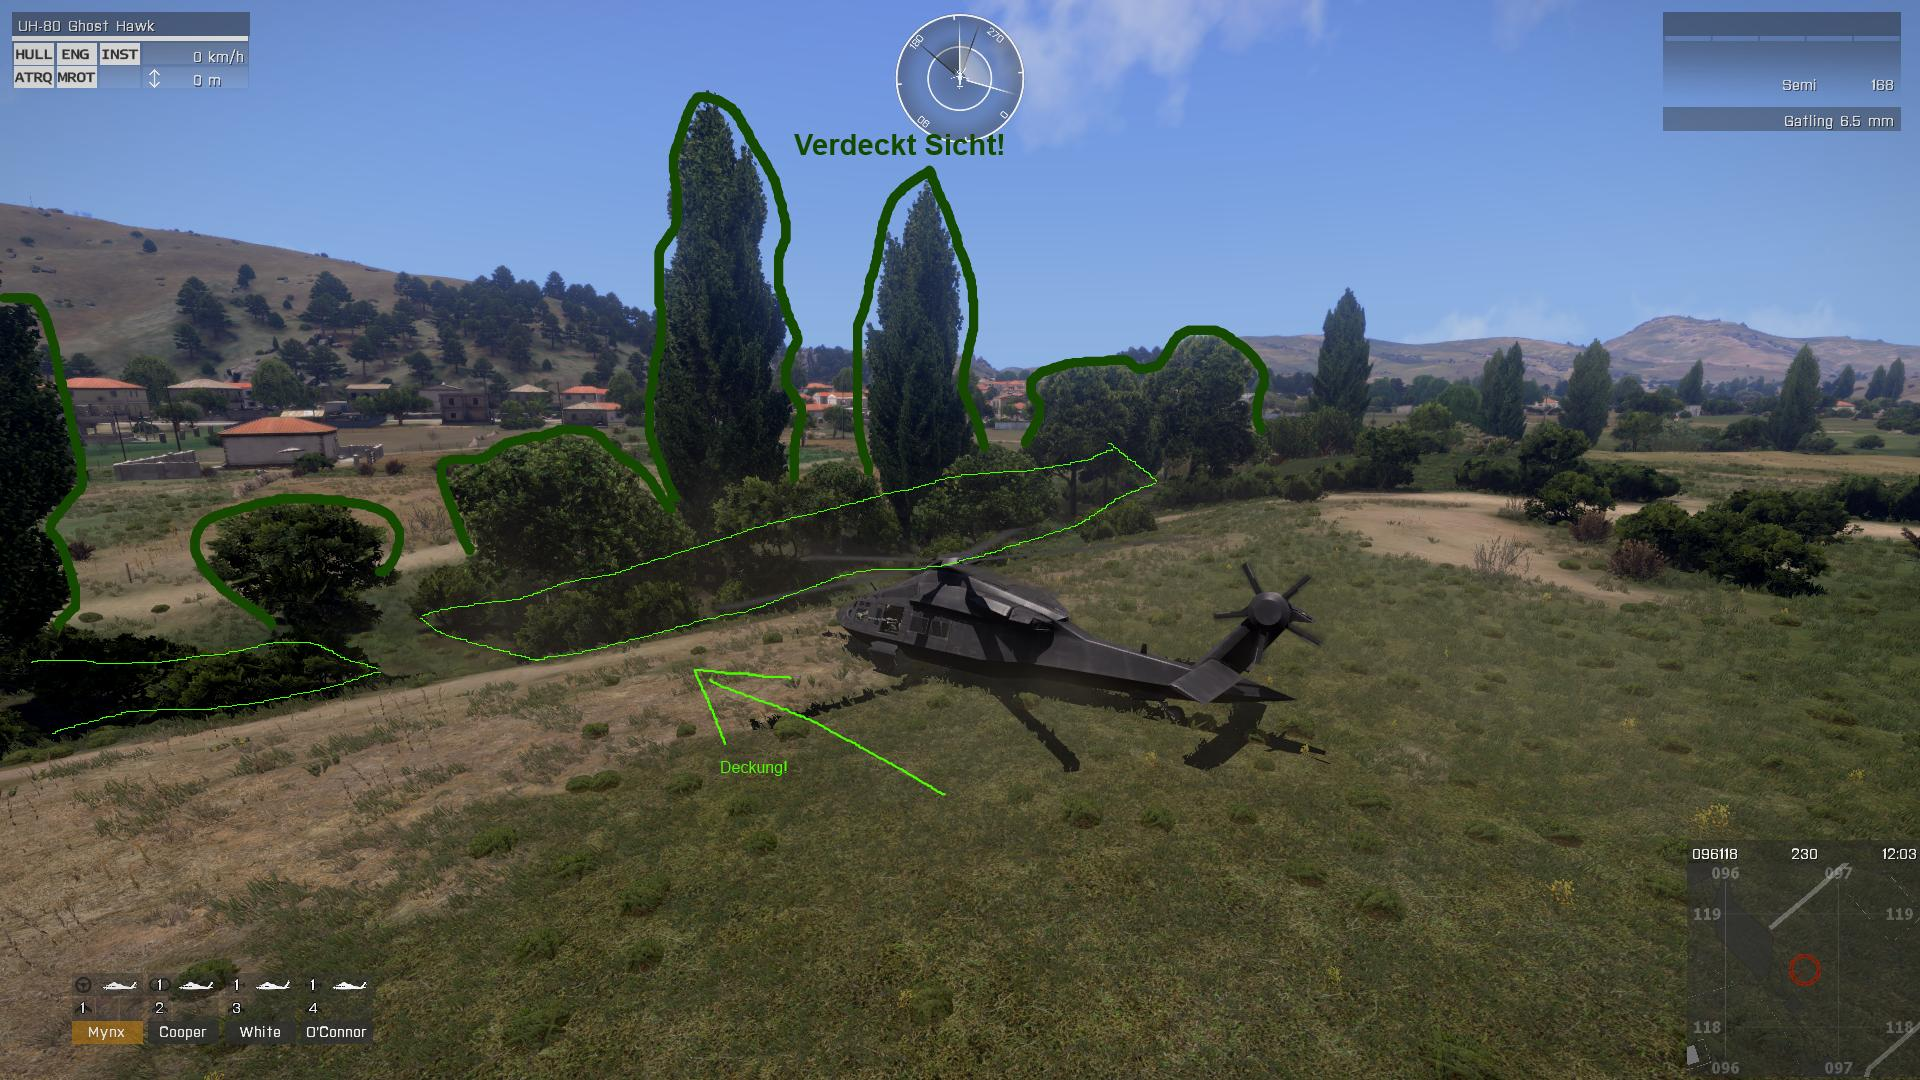
\includegraphics[width=\textwidth]{./Grafiken/Hubschrauber/verdeckteLandungamSammelpunktmitDeckung.jpg}
	\end{minipage}

	\begin{minipage}[t]{1\textwidth}
		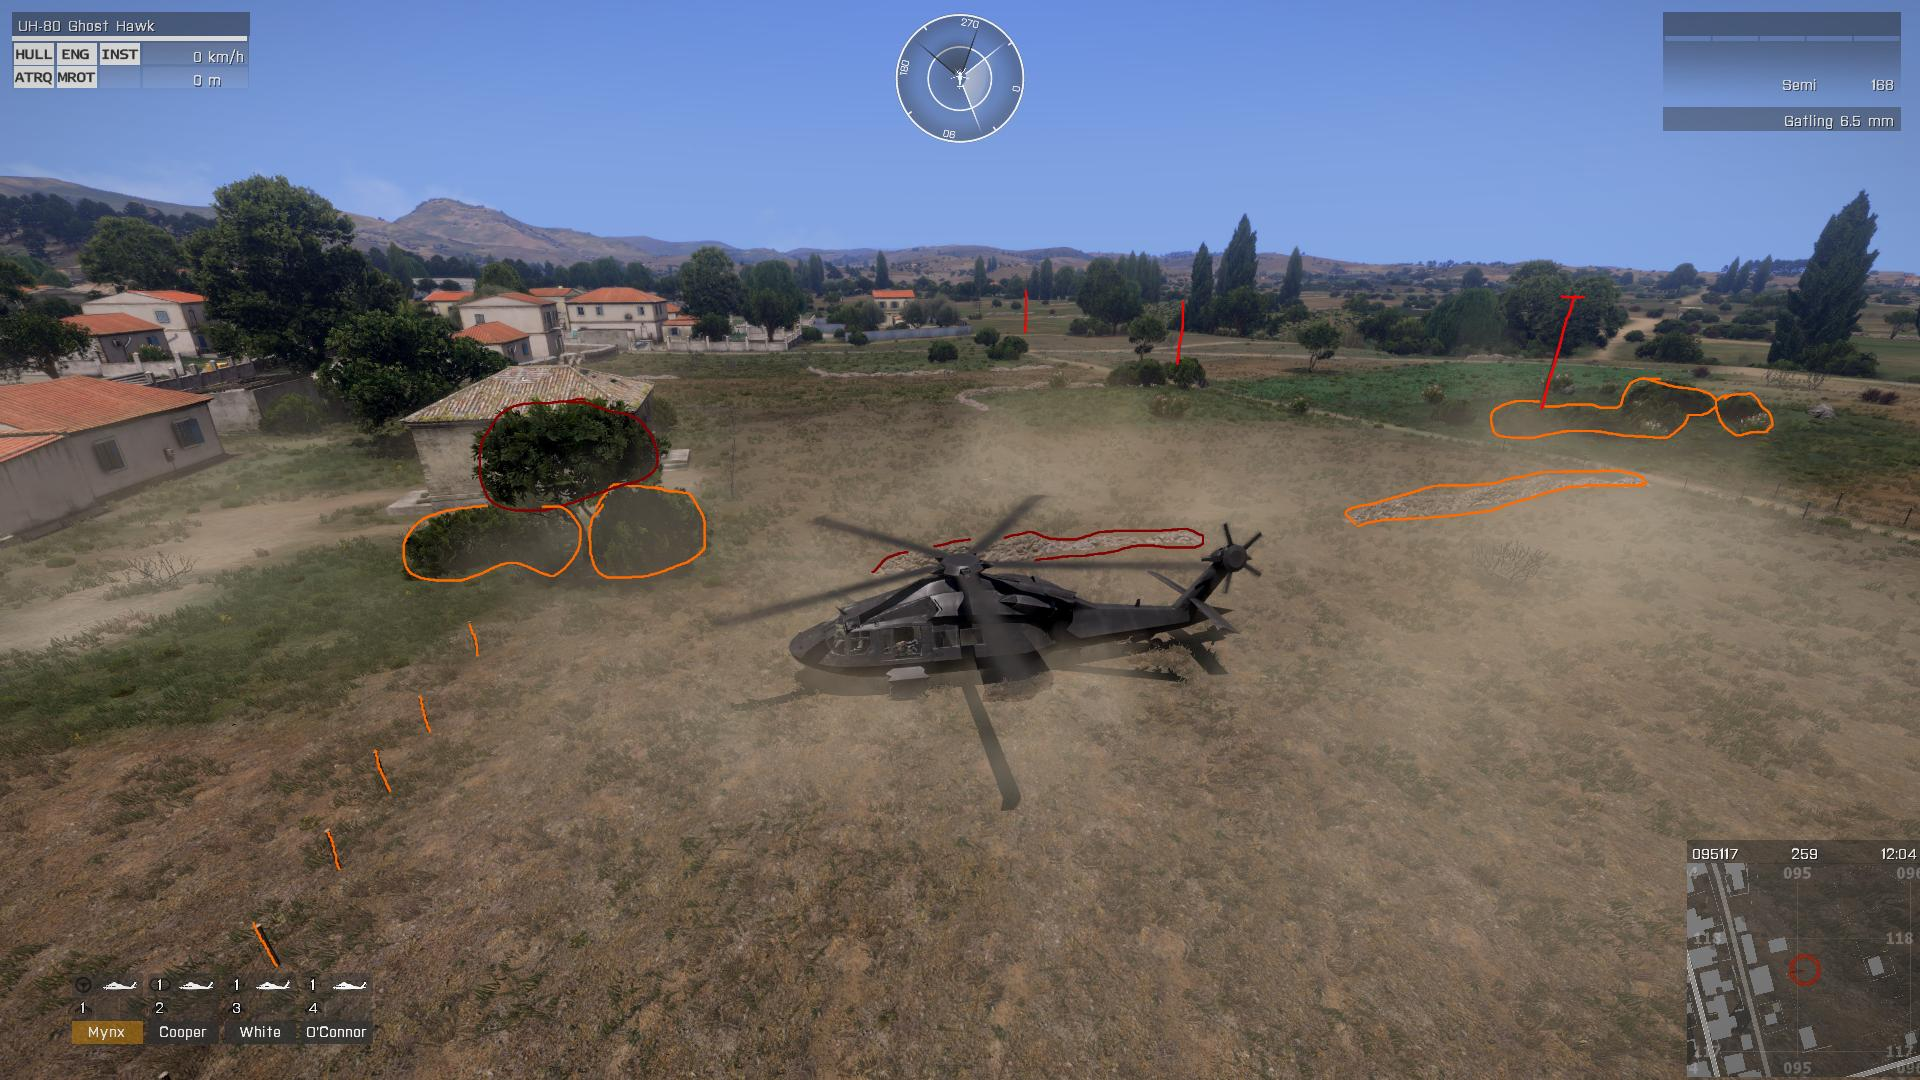
\includegraphics[width=\textwidth]{./Grafiken/Hubschrauber/BodenLesenausSichtdesPiloten1.jpg}
	\end{minipage}

	\begin{minipage}[t]{1\textwidth}
		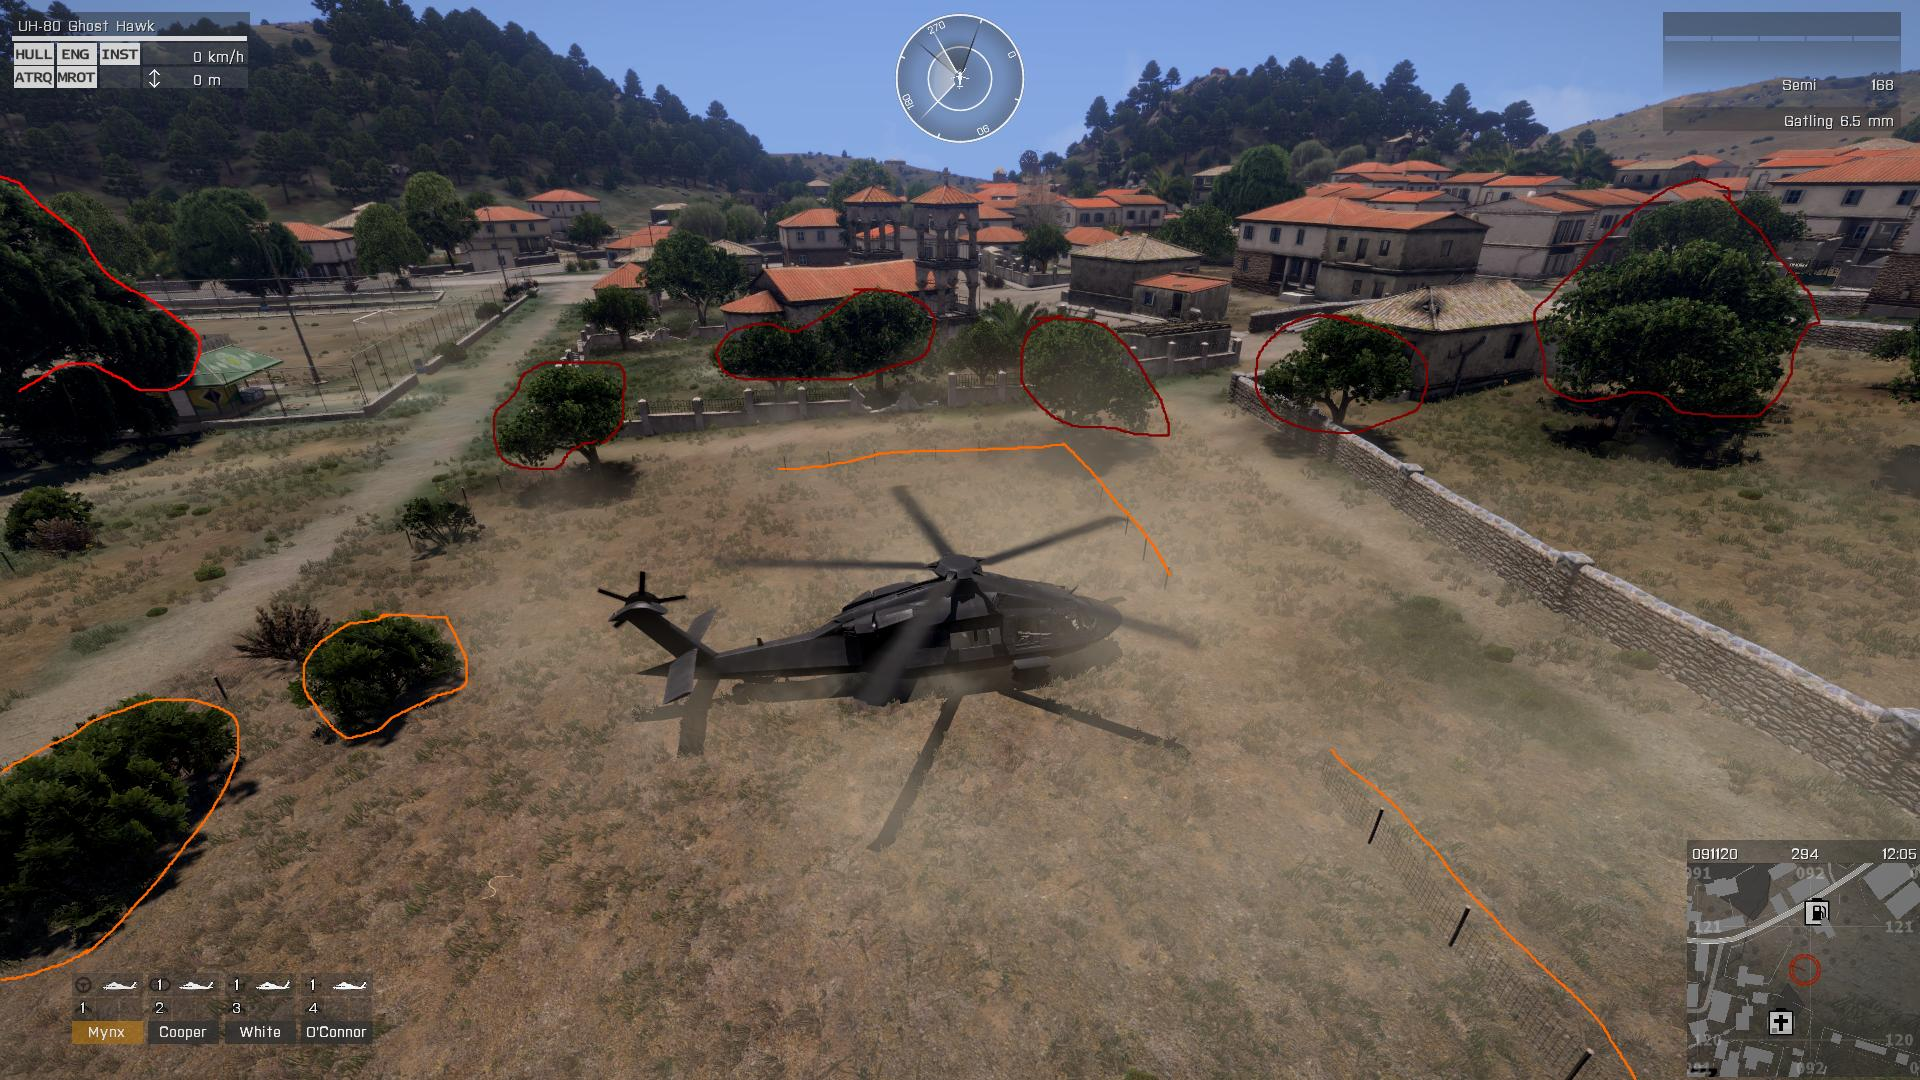
\includegraphics[width=\textwidth]{./Grafiken/Hubschrauber/BodenLesenausSichtdesPiloten2.jpg}
	\end{minipage}	

	Weiterhin sollten alle möglichen Gefahren im Bereich der Landezone analysiert werden. Gibt es feindl. Patrouillen im Gebiet? Sind Anti-Air Waffen des Feindes im Gebiet gemeldet worden? \\

	\begin{minipage}[t]{1\textwidth}
		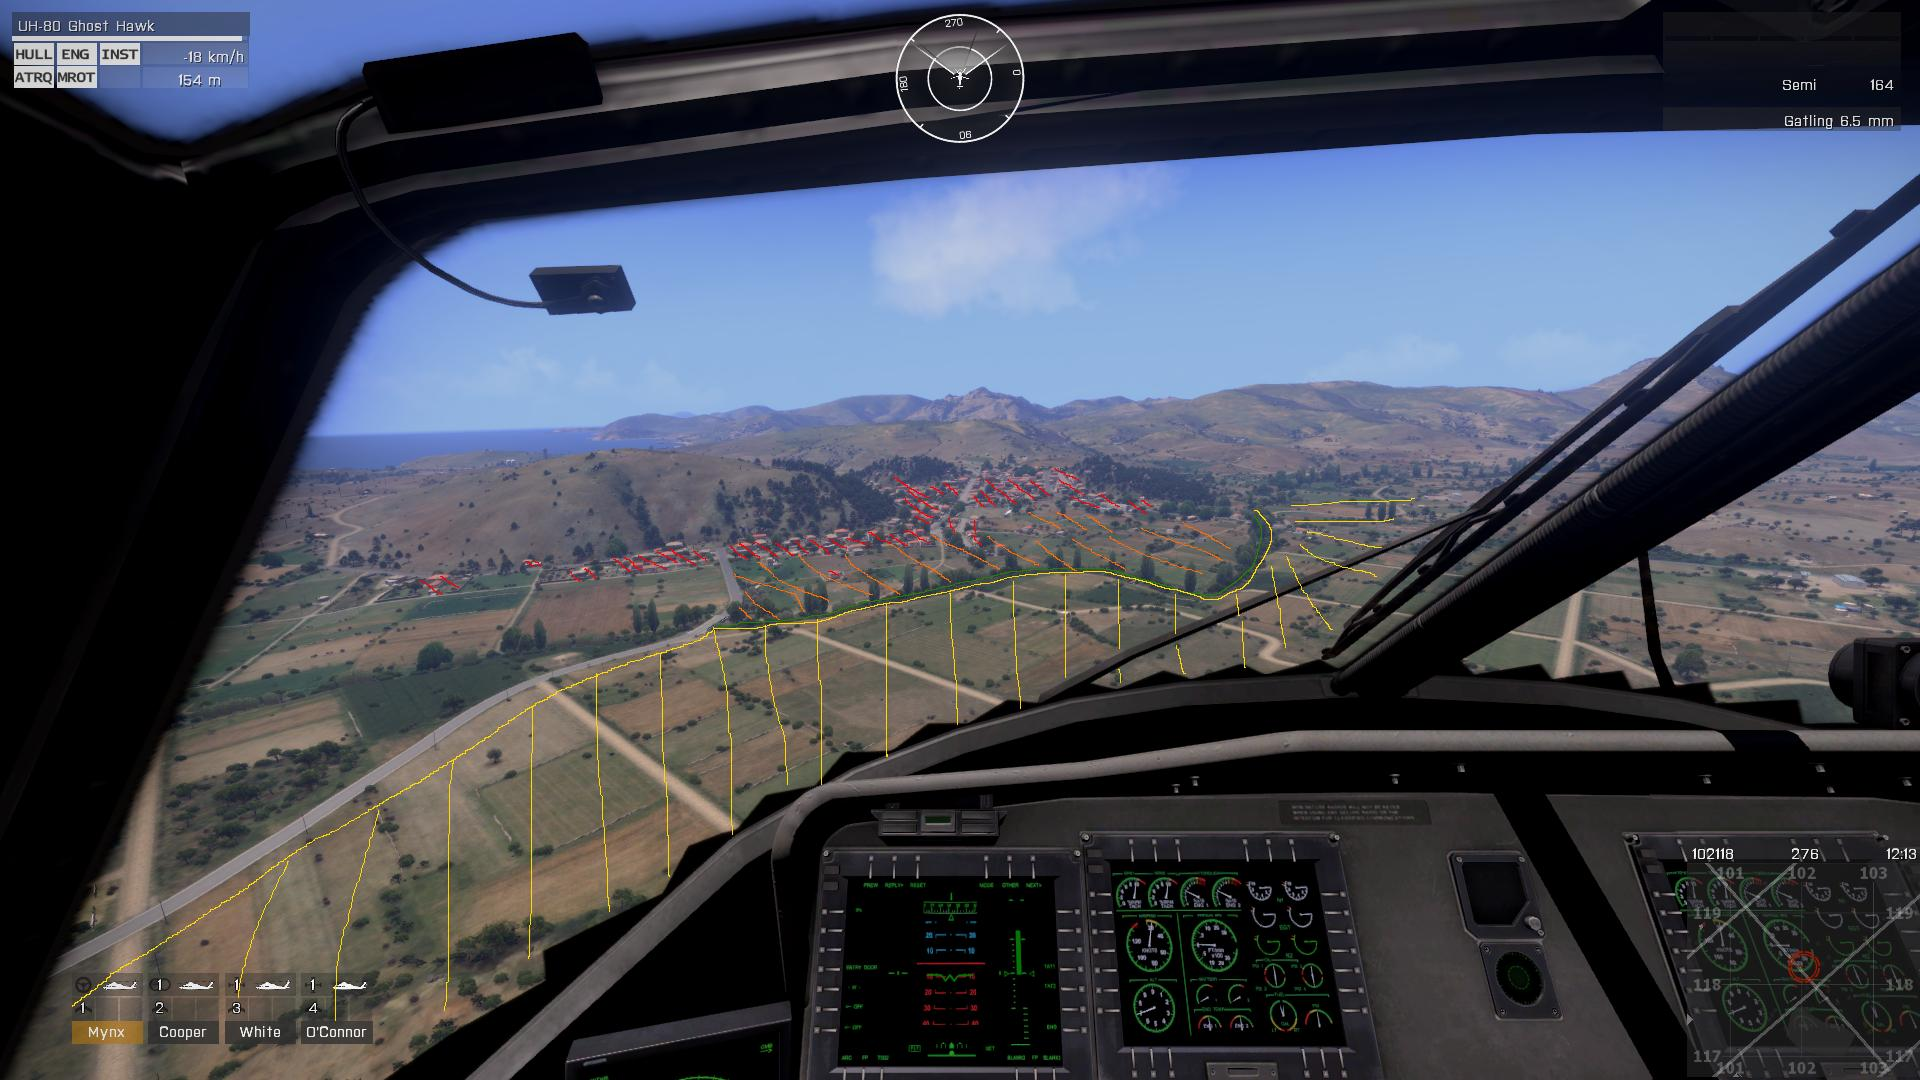
\includegraphics[width=\textwidth]{./Grafiken/Hubschrauber/AusSichtdesPiloten.jpg}
	\end{minipage}	
			
	Zum Abschluss wird eine Ersatz \ac{LZ} geplant und vermerkt. Sollte irgendetwas unvorhergesehenes passieren kann problemlos auf diese ausgewichen werden.

\subsection{Extraktion per Hubschrauber}
 	\begin{itemize} 
		\item Wenn die Landezone ausgesucht und definiert wurde, wird der Hubschrauber angefordert. Der Hubschrauber nimmt Kontakt per Funk auf, wenn er in das Gebiet des Trupps kommt und fordert die benötigten Maßnahmen an.

		\item Sobald der Hubschrauber in Reichweite ist, ist er auch in der Verantwortung des Infanterietrupps, welcher ihn angefordert hat. Die Infanterie muss den Hubschrauber um jeden Preis schützen!

		\item Sobald die Funk-Kommunikation hergestellt wurde muss der Hubschrauber mit Informationen vom Squadleader versorgt werden. Stichwort: Situationsbericht. Ist die Landezone Heiß/Kalt? Gibt es Bedrohungen im Gebiet die vorher nicht bekannt waren?

		\item Eine Basislandmarke, welche bei der Orientierung zur Suche der Landezone helfen kann, ist empfehlenswert. (Beispiel: Nördlich vom Sportplatz/Kirche)

		\item Wenn der Heli an einem etwas weiteren Ort entfernt sicherer landen kann und die Infanterie dafür etwas laufen muss ist das ein durchaus akzeptables Risiko.

		\item Wird eine spezielle Landezone gewählt oder muss unkonventionell gelandet werden sind die Gründe des Manövers dem Piloten mitzuteilen. (Wir landen am Südhang, da von Norden mit Feindfeuer zu rechnen ist.)

		\item Wenn der Hubschrauber Rauch verlangt wird dieser geworfen und wenn verfügbar/benötigt macht sich der Einweiser bereit.

		\item Der Hubschrauber meldet den Touchdown über Funk.

		\item Ghosthawk: Im finalen Anflug geben die Türschützen unterdrückungsfeuer auf jegliche Bedrohungen. Es wird so lange geschossen, bis der Hubschrauber den Boden berührt. Dann nur noch im Notfall. Sobald der Hubschrauber wieder abgehoben hat, wird das Unterdrückungsfeuer wieder aufgenommen.

		\item Die Annäherung an den Hubschrauber erfolgt frontal, mit einem finalen Schwenk zum seitlichen Einstieg. Dies bietet mehr Sicherheit und Schutz, ebenfalls wird dadurch Kreuzfeuer der Türschützen vermieden.

		\item >>Loadmaster<< gibt Pilot Freigabe. (oder Squadleader, je nach Truppstruktur/Verladestruktur)
	\end{itemize}

\subsection{Eingeflogen werden}
	\begin{itemize} 
		\item Der Pilot wurde über die \ac{LZ} informiert. Die Verantwortungsbereiche sind verteilt. Dann wird ein Sammelpunkt nahe der \ac{LZ} für den Abgesetzten Trupp definiert. Sobald der Infanterietrupp abgeladen wurde, wird sich unverzüglich zum Sammelpunkt begeben.

		\item Höchste Aufmerksamkeit beim finalen Anflug.

		\item Helikopter mit Seitenbewaffnung: Die Türschützen übernehmen das Unterdrückungsfeuer bis der Hubschrauber den Boden berührt.

		\item Der Pilot bespricht mit dem Loadmaster den Touchdown.

		\item Die Infanterie gibt ihr grünes Licht, das alle abgesessen haben und der Hubschrauber startet durch.

		\item Zeitfaustregel: Unter 1 Min. für ein Platoon!
	\end{itemize}

\subsection{Das Worst Case Szenario}
	\begin{itemize}
		\item \ac{LZ} Abbruch obliegt dem Piloten!
		\item Pilot hat das aller letzte Wort!
		\item Unter plötzlichem Beschuss die Deckung des Hubschraubers wenn nötig mit Rauch unterstützen.
		\item Wenn der Pilot einen Notfall deklariert, werden alle Pläne/Aktionen verworfen und das Sichern des Überlebens wird Priorität Nummer 1!
	\end{itemize}

\subsection{Finale Informationen zum Anweiser}
	Der Einweiser ist der Draht zum Hubschrauber.

	Wenn der Einweiser im Einsatz ist, ist dieser für den Hubschrauber verantwortlich. Dies bedeutet ebenfalls bei schwierigem Gelände dieses zu überwachen und bei Gefahr einen >>Abbruch!<< Befehl zu geben. In diesem Fall wird das Landemanöver abgebrochen und mit Rücksprache ein Neues einzuleiten.

\subsection{Beispielablaufplan: Anrufen eines Transportes}
	\begin{itemize}
		\item \ac{KT} funkt mit OPL Transportanfrage aus

    		\item \ac{OPL} gibt Transportfreigabe - erteilt Ausführungsbefehl

    		\item KT >>Anweiser<< nimmt gemeinsam mit Hubschrauber auf Hubschrauber \ac{SR} Kontakt auf

    		\item Absprache Auftrag Trupp mit Hubschrauber - Landmarke/Anflug

		\item  Hubschrauber meldet Anflug

    		\item Hubschrauber fordert ggf. Rauchmarkierung

    		\item Hubschrauber fordert Anweisung

    		\item Touchdown

    		\item Aufsitzen

    		\item >>Kampftrupp komplett.<< / >>Los! Los! Los!<< vom Truppführer

    		\item Abflug (Anweiser Verantwortung endet)
	\end{itemize}

\subsection{Santitätssystem}
\subsection{Konvoi}

%Mods
\newpage
\section{Mods}%\subsection{Task Force Arrowhead Radio (TFAR)}
\label{TFAR}
\subsubsection{Tastaturkürzel}
\begin{longtable}{|p{2cm}|p{5 cm}||p{2cm}|p{4cm}|} 
	\caption[Trupp]{die wichtigsten Tasten TFAR Tasten} \\ 
	\hline
	\cellcolor{backcolor} \textbf{Taste} & \textbf{Beschreibung} & \cellcolor{backcolor}\textbf{Taste} & \textbf{Beschreibung}  \\ 
	\hline
	\cellcolor{backcolor} STRG + P & SR Funkgerät öffnen & \cellcolor{backcolor}  ALT + P &  LR Funkgerät öffnen \\
	\hline
	\cellcolor{backcolor} PTT im TS\footnote{Push to Talk bzw. Spracherkennung im Teamspeak} & direkt sprechen & \cellcolor{backcolor}  Caps Lock & Auf SR Funk funken \\
	 \hline
	\cellcolor{backcolor} T & Aud SR Additional Channel funken & \cellcolor{backcolor}  Y & Auf LR Additional Channel funken \\
	 \hline
	\cellcolor{backcolor} STRG + TAB & Gesprächslautstärke einstellen\footnote{whispering / normal / yelling} & \cellcolor{backcolor}  & \\
	 \hline
	\cellcolor{backcolor} SHIFT + P & Unterwasserfunkgerät & \cellcolor{backcolor}  STRG + \~ & Auf Unterwasserfunk funken \\
	 \hline
\end{longtable}
\subsubsection{Short Range Funkgerät (AN/PRC – 152)}

	\begin{minipage} [b]{0.4\textwidth}
		\begin{enumerate}
			\item Lautstärke einstellen
			\item aktueller Kanal
			\item aktuelle Funkfrequenz
			\item Stereo Einstellungen (linkes Ohr / rechtes Ohr)
			\item Tastenfeld zur Eingabe der Funkfrequenz
			\item Frequenz löschen
			\item Frequenz bestätigen
			\item Funk kanal wechseln
			\item umschalten zwischen Lautsprecher und Kopfhörer
			\item Additional Channel festlegen
		\end{enumerate}
	\end{minipage}
	\begin{minipage}[t]{0.4\textwidth}
		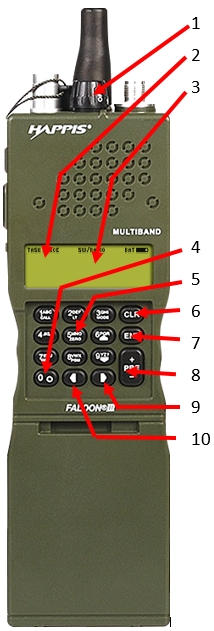
\includegraphics[width=\textwidth]{./Grafiken/Abschnitt/TFAR_SR_Radio.png}
	\end{minipage}


\subsubsection{Long Range Funkgerät (RT-15236 (ASIP) - LR)}
\begin{minipage}[t]{1\textwidth}
	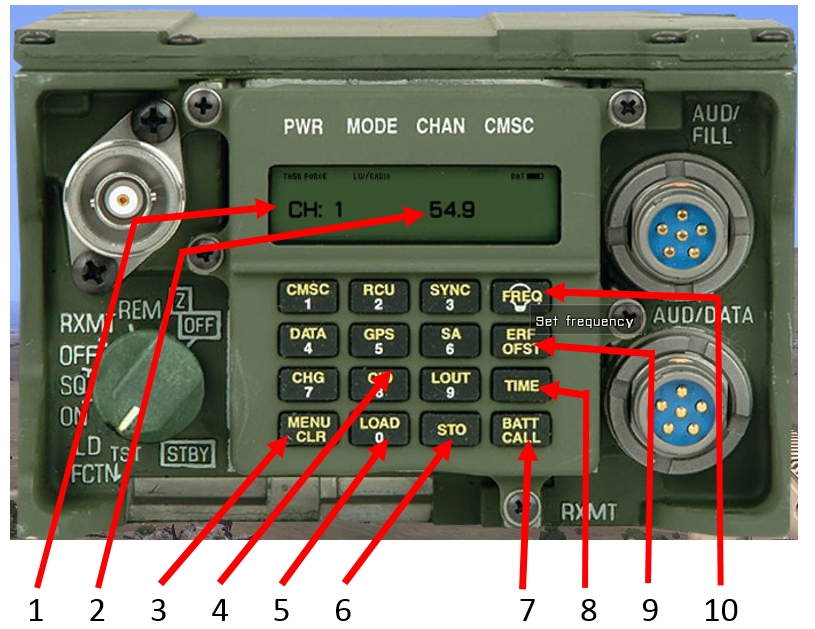
\includegraphics[width=\textwidth]{./Grafiken/Abschnitt/TFAR_LR_Radio.png}
\end{minipage}
\begin{enumerate}
	\item aktueller Kanal
	\item aktuelle Funkfrequenz
	\item Frequenz löschen
	\item Tastenfeld zur Eingabe der Funkfrequenz
	\item umschalten zwischen Lautsprecher und Kopfhörer
	\item Stereo Einstellungen (linkes Ohr / rechtes Ohr)
	\item Lautstärke  senken
	\item Lautstärke erhöhen
	\item Additional Channel festlegen
	\item Frequenz bestätigen
\end{enumerate}


%Sonstiges
\newpage
%\begin{landscape} %Querformat
\section{nützliche Tastatur (Um)Belegung}
%\end{landscape}
\newpage
\section{Umgang mit der Karte}
\newpage
\section{Die Bewaffnung}
\subsection{G36-Visier}
Seit wir das G36 haben, haben wir auch endlich wieder vernünftige Markierungen im optischen Visier. Damit braucht ihr als Schütze auch keine Rangefinder mehr - das ist alles <<all-ink>>. Erklärung anbei. Bei uns sieht die Strichplatte etwas anders aus, die Funktionen sind die gleichen. \\
\begin{minipage}[t]{1\textwidth}
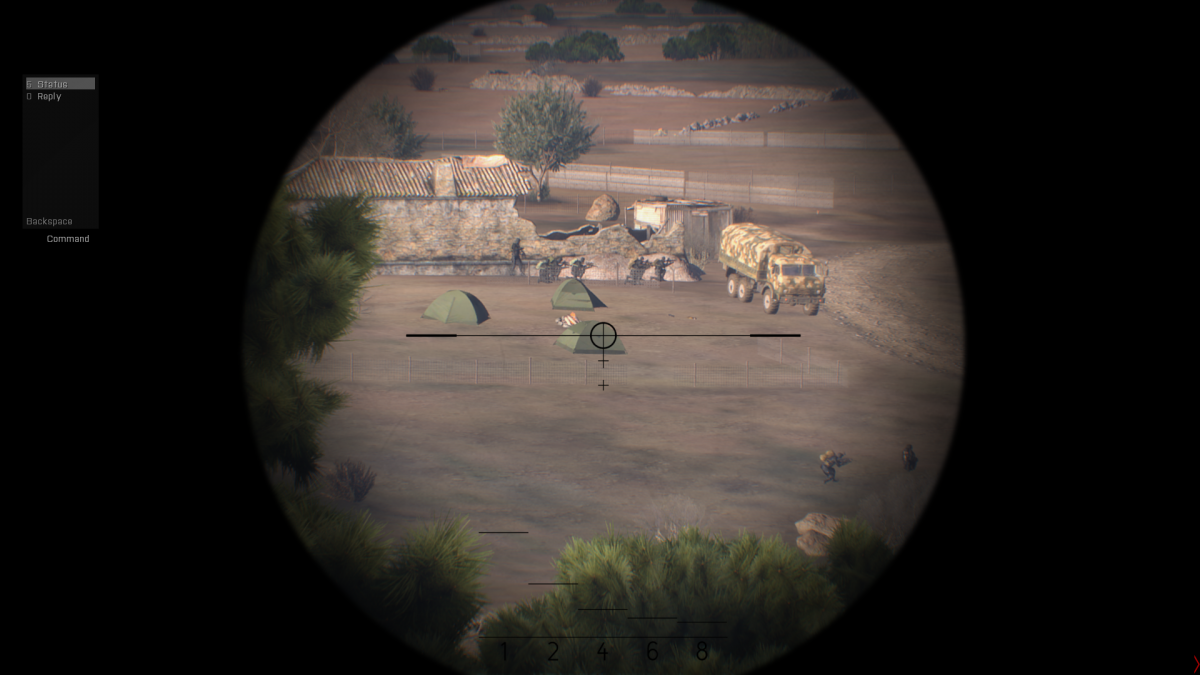
\includegraphics[width=\textwidth]{./Grafiken/Abschnitt/G36_teaser.png}
\end{minipage}
\begin{minipage}[t]{1\textwidth}
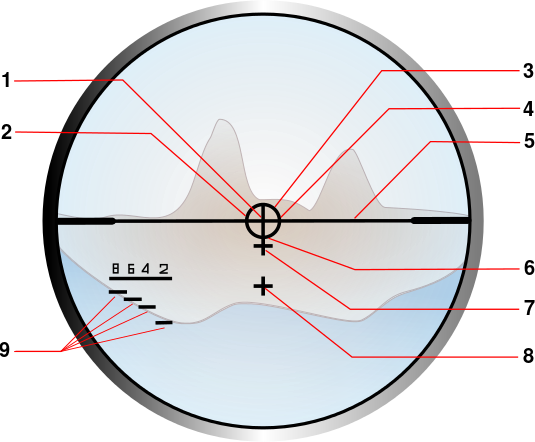
\includegraphics[width=\textwidth]{./Grafiken/Abschnitt/G36_Visier.png}
\end{minipage}
\begin{enumerate}
\item Zielmarke 200 m
\item Vorhaltemarke links bei Zielgeschwindigkeit von ca. 8 km/h bei 200 m Entfernung
\item Zielkreis (Innerer Durchmesser Schätzmarke 1,75 m Zielhöhe auf 400 m)
\item Vorhaltemarke rechts bei Zielgeschwindigkeit von ca. 8 km/h bei 200 m Entfernung
\item Horizontale Linie zur Verkantungserkennung
\item Zielmarke ca. 400 m
\item Zielmarke 600 m
\item Zielmarke 800 m
\item Entfernungsschätzmarken für Zielhöhe 1,75 m bei Entfernung X (200, 400, 600, 800m)
\end{enumerate}

\subsection{Das G36}
Das G36 ist eineStandard Infanterie Waffe. Ihre optimale Einsatzreichweite liegt bei ca. 100-400 m \\
Grenadiere, Truppführer sowie ihre Funker verfügen über ein G36 mit zusätzlichem Unterlaufgranatwerfer. Dieser wird durch umschalten mit der Feuermodi Taste (F) erreicht. Durch drücken von \glqq Bild hoch\grqq und \glqq Bild runter\grqq wird die Entfernung eingestellt (50-350 m). Der Unterlaufgranatwerfer stellt damit eine hervorragende Waffe da um Feindverbände zu unterdrücken und weiter entfernte Ziele mit Rauchgranaten zu markieren. \\

\subsection{Das MG5 (HK121)}
Das Maschinengewehr 5 wird im Verbund mit einem MG Assistenten eingesetzt. Das MG5 ist eine der effektivsten Waffen zur Infanteriebekämpfung. Das Visier entspricht dem G36. Seine schwere 7,62 mm Munition kann auch Gebäude oder leichte Deckung durchschlagen. Bevorzugt sollte das MG5 im Liegen und aufgelegt eingesetzt werden. Der MG-Assistent trägt die Munition und sichert den MG-Schützen mit ab. Das MG5 verfügt über drei Feuermodi, die unterschiedliche Feuerraten und damit unterschiedliche Präzision anbieten.  (ca. 600  / 700 / 800 Schuss /min) \\

\subsection{Das Panzerfaust 3 Visier}
Die Panzerfaust 3 ist unsere Standard AT (Anti-Tank) Waffe und wird gegen stark gepanzerte Fahrzeuge eingesetzt. Im Visier sind 5 Distanzmarken eingezeichnet. Von Unter 100 - 400 Meter. Die Panzerfaust 3 wird rein optisch gezielt, es gibt keine Zielführung oder "Lock On" wie bei manchen anderen AT Waffen. \\
 Ein statisches Ziel sollte zwischen den linken und rechten Balken möglichst eingegrenzt werden, so dass das Mittlere + etwa auf der Höhe des Turms ausgerichtet ist. Ist das Ziel im Nahbereich (< 100m), genügt es das oberste, eingekreiste Plus bzw. dessen Führungslinie zu verwenden. Bewegt sich das Fahrzeug nach Links oder Rechts weg, ist das jeweilige der Richtung entgegensetzte + zu verwenden, da das Geschoß je nach Distanz verzögert eintrifft. \\
\begin{minipage}[t]{1\textwidth}
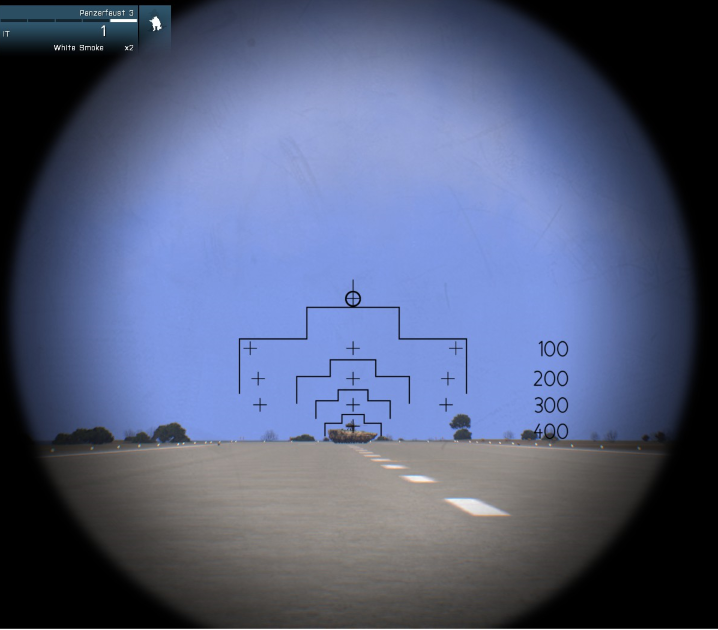
\includegraphics[width=\textwidth]{./Grafiken/Abschnitt/Panzerfaust_Visier.png}
\end{minipage}

\subsection{Die Panzerfaust 3}
Die Panzerfaust 3 ist eine Einwegwaffe. Zur Reduzierung der Sichtbarkeit kann der Gefechtskopf beim Transport entfernt werden. Beim Einsatz der Panzerfaust 3 ist zu beachten dass diese eine Rückstrahlzone hat in der befreundete Einheiten verletzt werden können. Diese Rückstrahlzone ist minimiert aber vorhanden. Um sicherzustellen das keine befreundeten Einheiten sich in dieser Rückstrahlzone befinden wird die PZF3 auf das Ziel ausgerichtet und gefragt ob die 
\glqq Rückstrahlzone frei?\grqq ~ ist. Anwesende Einheiten überprüfen dann ob diese frei ist und geben dann die Freigabe \glqq Rückstrahlzone frei!\grqq. Die Panzerfaust bleibt dabei immer auf den Feind (oder erwarteten Feind gerichtet).  Mit der Panzerfaust 3 kann fast jedes Fahrzeug mit einem Schuss zerstört werden. \\

\subsection{Das Fliegerfaust 2 Stinger Visier}
Die Fliegerfaust ist unsere Standard \acf{AA} Waffe. Sie wird vor allem gegen niedrigfliegende feindliche Hubschrauber und Drohnen eingesetzt, kann aber auch gegen Flugzeuge wirken. Ihre Maximalreichweite beträgt ca. 6km, die maximale Flughöhe des Ziels ist < 2km. \\
Die Fliegerfaust hat ein relativ simples optisches "Guckloch" Visier, welches zur optischen Zielerfassung dient, jedoch nicht unbedingt für die Zielerfassung erforderlich ist. Für die Zielerfassung wird ein "Lock-On" System verwendet, sprich man muss die Fliegerfast auf das Ziel ausrichten, danach drückt man T (Lock Target Taste) und erhält einen wiederholenden Ton, der anzeigt, das das Ziel erfasst wird. Sobald die Fliegerfaust das Ziel endgültig erfasst hat erhöht sich die Frequenz und Wiederholrate dieses Tons und man kann den Abzug betätigen. Je weiter ein Ziel entfernt ist, desto wirksamer sind die vom Ziel eventuell eingesetzten Gegenmaßnahmen, es empfiehlt sich generell immer sofort nachzuladen und einen nachfolgenden Schuss abzusetzen. \\
\begin{minipage}[t]{1\textwidth}
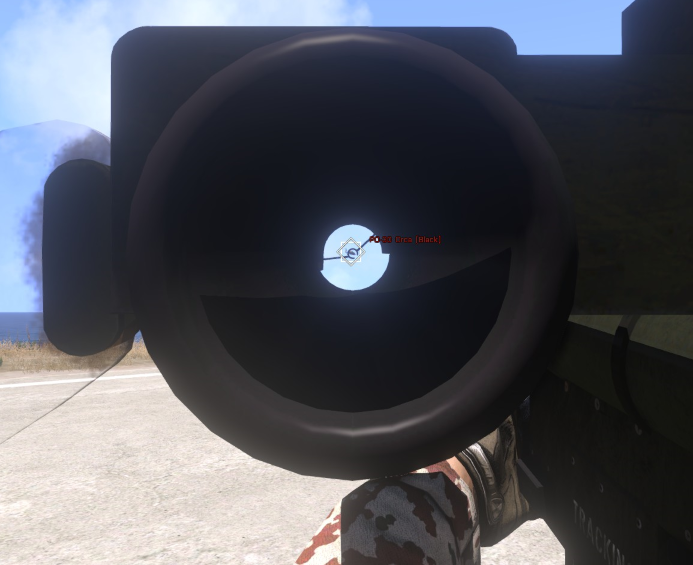
\includegraphics[width=\textwidth]{./Grafiken/Abschnitt/Fliegerfaust_Visier.png}
\end{minipage}

\subsection{Die Fliegerfaust}
Sie wird selten im \ac{TTT} eingesetzt da die meisten Terroristischen Feindverbände über keine Flugeinheiten verfügen bzw. diese durch die Flugeinheiten bekämpft werden. Es gelten die gleichen Regeln für die Rückstrahlzone wie bei der Panzerfaust 3.\\

\subsection{Granaten}
Jeder Infanterist verfügt über Spreng-, Rauch-, Blend- und \acf{IR}-Granaten. Zusätzlich (Aufgrund der Verwendung) Knicklichter. Der Einsatz von Granaten sollte sorgfältig überlegt sein. \\
Rauchgranaten sollten entsprechend ihrer Rauchfarbe eingesetzt werden. Individuell kann ein anderer (Farb-) Einsatz abgesprochen werden. Ein kleiner Hinweis das man, und auch welche, Granate man einsetzt hat sicherlich noch niemanden geschadet. Ein typisches Problem ist auch das Rauchgranaten eher zu selten als zu oft eingesetzt werden. \\
\\
\begin{tabular} {|p{0.25\linewidth}|p{0.65\linewidth}|} \hline
Roter Rauch		& Markierung von Feinden\\ \hline
Grüner Rauch	& Markierung der eigenen Stellung \\ \hline
Grauer Rauch	& Einnebeln der eigenen Stellung um unerkannt anzugreifen oder sich zurückzuziehen\\ \hline 
Violetter Rauch & Markierung von Landezonen \\ \hline
\end{tabular}\\
\\
\ac{IR}-Granaten dienen der Markierung von Gebieten (bei Nacht) um zum Beispiel \ac{CAS} einzuweisen. \ac{IR}-Granaten sind deutlich sichtbar für jedes Nachtsichtgerät! \ac{IR}-Granaten und Knicklichter können auch mittels \ac{CSE} Menü am Körper angebracht werden.

\subsection{Sonderbewaffnung}
Sonderbewaffnung sind den Spezialisten Trupps überlassen und stellen damit nicht den Teil der \ac{AGA} dar. Sonderbewaffnungen bedürfen einer Speziellen Grundausbildung (\ac{SGA}). Erwähnt seien hier die Minen und Sprengsätze von Pionieren, Drohen der \ac{UAV}-Operatoren, Scharfschützengewehre und Mörser. \\



%das Abkürzungsverzeichnis erstellen
\pagebreak
\section*{Abkürzungsverzeichnis}
\addcontentsline{toc}{section}{Abk\"urzungsverzeichnis} 
\begin{acronym}[SEPSEPSEP]
\setlength{\itemsep}{1em}
	\acro{AAR}{After Action Report}
	\acro{OPL}{Operationsleitung}
	\acro{SQL}{Squadlead}
	\acro{FAC}{Forward Air Controler}
	\acro{AT}{Anti Tank}
	\acro{UAV}{Unmanned Aerial Vehicle}
	\acro{TTT}{Tactical Training Team}
	\acro{AA}{Anti Air}
	\acro{KPZ}{Kampfpanzer}	
	\acro{SPZ}{Schützenpanzer}
	\acro{CAS}{Close Air Support}
	\acro{CQB}{Operationsleitung}
	\acro{AGA}{Allgemeine Grundausbildung}
	\acro{SGA}{Spezielle Grundausbildung}
	\acro{KSK}{Kommando Spezialkräfte}
	\acro{MedEvac}{MEDical EVACuation}
	\acro{CSE}{Combat Space Enhancement}
	\acro{IR}{Infrarot}
	\acro{EOD}{Explosive Ordnance Disposal}
	\acro{LZ}{Landezone}
	\acro{KT}{Kampftrupp}
	\acro{SR}{Short Range}
	\acro{LR}{Long Range}
\end{acronym}
\pagebreak

%Ganz zum Schluß
\newpage
\section{Autoren}
	Die namentlich genannt werden wollen (und die ich noch auftreiben konnte). \\
	Ein herzliches Dank an euch für eure fleißige Mitarbeit, an alle die am \ac{TTT} mitwirken und Leuten wie mir es mal so richtig zeigen, also taktisches Spielen. \\
	(in chronologischer Reihenfolge) \\

\begin{tabular}{cc}
	grauer Wolf  					& 	Erstellung, Zusammenstellung und einiges aus dem AGA Handbuch \\
	Lufros 					& 	Funkhandbuch \\
	Mynx 						& 	Hubschrauber für Infanterie \\
	Relain						& 	Ersterstellung vieler Inhalte \\
	SCiite 						& 	Layout \\
	Stura 						& 	Abkürzungsverzeichnis \\

\end{tabular}


\cleardoublepage
\appendix

\listoftables
\addcontentsline{toc}{section}{Tabellenverzeichnis}


\end{document}